\chapter{数据更新} \label{chp:数据更新}
数据更新工作在深圳市交通仿真系统(二期) 已有的\ppyear 年静态 GIS 数据
和动态交通数据基础上,根据 \pyear 年各类数据变化情况对底层数据进行更新,
将系统的输入数据时间更新至 \pyear 年。

数据更新工作是后续数据挖掘、数据查询系统更新以及模型系统更新的前提,
是一项重要的基础性工作。

\section{动态交通数据处理} \label{sec:动态交通数据处理}
动态交通数据指的是带有时间信息的交通数据, 可以通过数据本身来反映不
同时段交通的特征以及变化趋势。 其更新频率高,通常 1 分钟就会更新 2-5 次,
可以反映交通的实时状态和动态变化,因此称为动态数据。

深圳市交通仿真系统(二期)中囊括的动态交通数据包括出租车 GPS 数据、
公交车 GPS 数据、深圳通 IC 刷卡数据 (轨道和常规公交)、车牌识别数据四大类。
本项目的目标就是,将这四类数据从原始状态开始经过一系列技术加工, 最终更
新至符合深圳市交通仿真系统(二期)输入格式的标准化数据。

\subsection{原始数据采集}
动态交通数据来源于不同的单位,因此数据采集工作就是按照一定的时间周
期从这些单位获取到最新的原始数据。

本项目按季度分别从市交委、市交警局监控中心、东部公交公司、西部公交
公司、 巴士集团公司、 深圳通公司、地铁 ACC 公司通过现场拷贝、网络传输和光
盘邮寄几种方式获取所需数据。 本项目已采集的原始动态数据至 \pyear 年 12 月。

\smalltitle{公交刷卡数据}
\begin{longtabu} to \textwidth {|c|X[1,l]|}
\hline
数据内容 & 包括每日350万次公交刷卡的线路、站点、时间、车牌以及卡号等信息\\\hline
数据大小 & \pyear 年全年数据大小约 14GB\\\hline
数据格式 & ASCII 文本格式\\\hline
数据来源 & 深圳通公司\\\hline
采集方式 & 每季度由深圳通公司将当季度数据刻录光盘, 再派指定人员取回\\
\hline
\end{longtabu}
\addtocounter{table}{-1} % 不需要计数

\smalltitle{轨道刷卡数据}
\begin{table}[ht]
\centering
\begin{tabularx}{\textwidth}{|c|X|}
\hline
数据内容 & 包括轨道刷卡和投币每日650万次的进出站点、时间和卡号信息\\\hline
数据大小 & \pyear 年全年数据大小约 15GB\\\hline
数据格式 & ASCII 文本格式\\\hline
数据来源 & 地铁ACC公司\\\hline
采集方式 & 每季度由 ACC 公司将当季度数据刻录光盘, 再派指定人员取回\\
\hline
\end{tabularx}
\end{table}

\smalltitle{车牌识别数据}
\begin{table}[ht]
\centering
\begin{tabularx}{\textwidth}{|c|X|}
\hline
数据内容 & 包括全市视频监测点和车牌识别系统提供的车牌识别数据\\\hline
数据大小 & \pyear 年全年数据大小约480GB\\\hline
数据格式 & ASCII 文本格式\\\hline
数据来源 & 市交警监控中心\\\hline
采集方式 & 每季度派指定人员去市交警监控中心现场拷贝\\
\hline
\end{tabularx}
\end{table}

\smalltitle{公交 GPS 数据}
\begin{table}[ht]
\centering
\begin{tabularx}{\textwidth}{|c|X|}
\hline
数据内容 & 包括按每 10 秒/回传频率的出租车运行 GPS 数据\\\hline
数据大小 & \pyear 年全年数据大小约 350GB\\\hline
数据格式 & ASCII 文本格式\\\hline
数据来源 & 市交委\\\hline
采集方式 & 每季度由专人去现场拷贝\\
\hline
\end{tabularx}
\end{table}

\subsection{数据预处理}
由于原始数据来源于不同的单位,原始数据的格式存在很大的差异,为达到
能够统一输入深圳市交通仿真系统(二期) 数据平台的要求, 需要按照原系统设
计的表格结构对数据进行字段顺序调整、精简和合并等预处理工作实现标准化,
本项目中针对每类数据的特点,开发了专门的程序进行处理,实现了自动化作业。
\tref{tbl:数据预处理工作}是每类数据处理的工作内容。

\begin{table}[ht]\centering
  \renewcommand\tabularxcolumn[1]{m{#1}}
  \caption{数据预处理工作\label{tbl:数据预处理工作}} 
  \begin{tabularx}{\textwidth}{|c|X|}
    \hline
    {\bfseries 数据类型} & \multicolumn{1}{c|}{\bfseries{预处理工作}}\\\hline
     公交刷卡数据 & 清理无效字符;按照系统表结构调整顺序\\\hline
     轨道刷卡数据 & 清理无效字符;按照系统表结构调整顺序\\\hline
     车牌识别数据 & 清理无效字符;合并成每天一个文件;按照系统表结构调整顺序\\\hline
     公交GPS数据 & 清理无效字符和错误数据;合并成每天一个文件;按照系统表结构调整顺序\\
    \hline
  \end{tabularx}
\end{table}
% 另外,为了后续计算道路车速、 公交车车速、 出租车 OD 和空重车等指标,
% 需要对出租车数据和公交 GPS 数据进行进一步的预标准化预处理, 所有的工作
% 都由专门开发的程序来自动化完成。

% \smalltitle{出租车 GPS 数据标准化}
% 预处理程序为 FCD\_SyncData-SZ,主要包括: 程序运行库、批处理程序
% statnew.bat 和配置文件 config.xml。操作步骤如下:

% \begin{nbeae}
% \item 设置输入文件路径\\
% \indenttext{建立两个文件夹,用于存放 GPS 原始数据和标准化后的 GPS 数据。例如,
% 在 E 盘根目录下建立文件夹“GPSINPUT”,“GPSOUTPUT”。将 GPS 原始数据
% 解压后放入“ GPSINPUT”下,文件放置规则需按照年月日顺序依次建立相应文
% 件夹,然后放入。如:\pyear 年 1 月 1 日数据,放置路径为
% “E:$\backslash$GPSINPUT$\backslash$\pyear$\backslash$1$\backslash$1$\backslash$”,
% \pyear 年 1 月 2 日数据,放置路径为“E:$\backslash$GPSINPUT$\backslash$\pyear
% $\backslash$1$\backslash$2$\backslash$”,其余数据依次类
% 推,将需标准化的 GPS 数据按照该规则放置到正确路径下即可。}
% \item 设置配置文件\\
% \indenttext{将 GPS 输入路径与输出路径写入系统配置文件“ config.xml”中。将配置文
% 件中如下部分正确填写即可。}\\
% \indenttext{<frompath> E://GPSINPUT//</frompath>}\\
% \indenttext{<topath> E://GPSOUTPUT//</topath>}\\
% \indenttext{Frompath 和 topath 标签中间的路径为需要填写的输入和输出文件路径。 路
% 径只需配置到“年”的上一级路径即可,如上示例中,“ 2015”文件夹上一级为
% “ GPSINPUT”,那么“ frompath”只需要配置为“ E://GPSINPUT//”即可。}
% \end{nbeae}

\subsection{分类集中存储} \label{subsec:分类集中存储}
预处理后的动态交通数据将通过 FTP 方式上传到数据挖掘主机(配置见附
录), 按照预先设定的分类目录进行集中存储,作为后续数据挖掘的输入。

预处理动态交通数据每季度上传一次,包含三个月,每月一周(周一至周日
7 天)的数据。在数据挖掘主机中,建立了以下原始数据目录结构,用于存放这
些数据。\fref{tbl:数据挖掘主机中分类集中存储文件的目录结构}是存储文件的目录结构。

\begin{table}[!ht]\centering
  \caption{数据挖掘主机中分类集中存储文件的目录结构\label{tbl:数据挖掘主机中分类集中存储文件的目录结构}} 
  \begin{tabularx}{\textwidth}{|Y|Y|Y|Y|Y|}
    \hline
    \multicolumn{1}{|c|}{\bfseries 根目录} & \multicolumn{1}{c|}{\bfseries 二级目录} & 
    \multicolumn{1}{c|}{\bfseries 三级目录} & \multicolumn{1}{c|}{\bfseries 四级目录} &
    \multicolumn{1}{c|}{}\\\hline
    \$DM\_HOME & 年份 & 季度 & 数据类型 & 文件\\
    \hline
  \end{tabularx}
\end{table}

其 中 , \$DM\_HOME 指 数 据 挖 掘 主 机 存 放 数 据 的 根 目 录 , 默 认 为
/home/dm/data。在根目录下, 每年数据存放在名称为“ 4 位年份”的二级目录中,
例如 2013、 2014、 2015。二级目录下创建四个三级目录,目录名称为: s+季度
( 1-4), 该子目录用于存放某年一个季度的数据。在三季目录下,按不同种类的
交通数据分别建立对应的四级目录:

\begin{para}
\item[目录 ic] 存储 IC 刷卡数据(包括轨道和巴士刷卡数据)
\item[目录 gps] 存储巴士 GPS 数据
\item[目录 lp] 存储车牌识别数据
\end{para}

在四级目录下, 按照每天一个文件的形式存放相应的数据文件。 如果原始数
据以压缩文件方式提供,在写入对应目录之间,必须先进行解压缩处理,然后才
写入目录。\fref{fig:分类集中存储后的目录结构}为分类集中存储后的目录结构截图。

\clearpage
\begin{figure}[!ht]
  \centering
%\begin{center}
  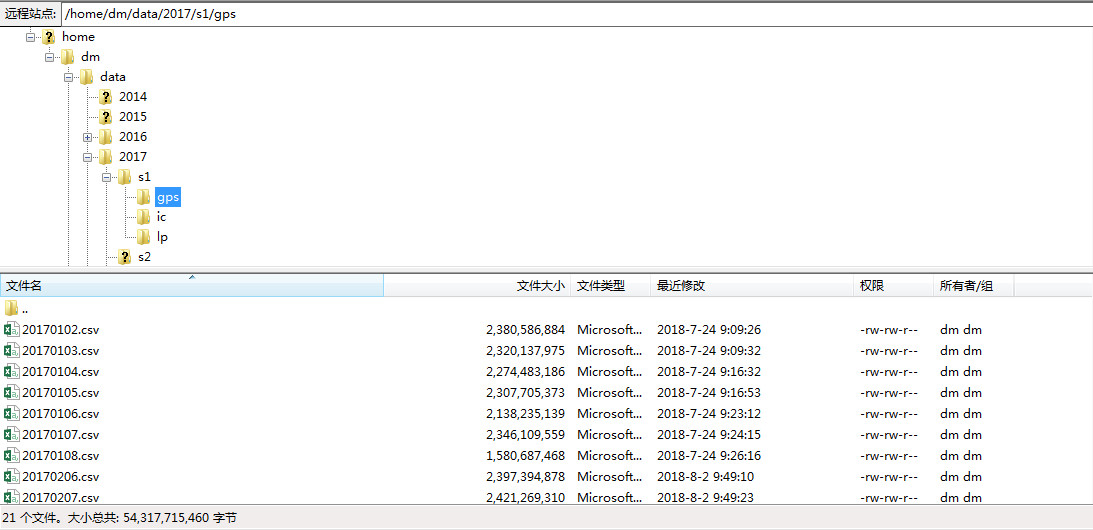
\includegraphics[width=\textwidth]{chp02_分类集中存储后的目录结构.jpg}
  \caption{分类集中存储后的目录结构\label{fig:分类集中存储后的目录结构}} 
%\end{center}   
\end{figure}

\section{静态 GIS 数据处理} \label{sec:静态GIS数据处理}
静态 GIS 数据指用于展示和分析的 GIS 图层数据, 包括各类区域边界、 道
路网络、公交网络站点的形状和属性信息等, 主要用于制作各类交通专题图、基
础统计以及辅助数据挖掘计算。 其变化频率低、 更新周期较长,一般为一年更新
一次,因此相对于动态交通数据的高更新频率来说属于静态数据。

\subsection{现有数据类型} \label{sec:现有数据类型}
深圳市交通仿真系统(二期) 中囊括的静态 GIS 数据包括: 基础 GIS 数据
(行政区、水系、绿地、法定图则、组团、街道),基层路网数据(道路节点、
路段、交通小区、主要节点数据),公交和轨道 GIS 数据(公交站点、公交网络、
轨道站点、轨道网络),调查数据(居民出行调查、轨道二期开通后调查、交叉
口/断面流量调查等),现状和规划土地利用(建筑物普查数据、规划一张图),
现状和规划人口岗位数据, POI 数据(医院、学校、口岸、火车站、飞机场、港
口、公共停车场、 检测器), 共 4 大类 26 小类。详细表信息见附表。

其中, 道路数据和公交数据涉及后续的数据挖掘系统输入,需要进行年度更
新,其他 GIS 数据根据需求不定期进行更新。 为了提高工作效率, 数据更新工
作按照不同 GIS 图层并行开展, 更新后的 GIS 数据以 shapefile 格式进行存储,
待后续数据挖掘和数据查询系统使用。

\subsection{道路数据更新}
道路数据更新的技术方法是:以市规划国土委(海洋局)信息中心提供的最
新版深圳市道路网络数据为底图,按照交通模型和查询的数据结构需求,采用
ArcGIS 软件在深圳市交通仿真系统(二期)已有的 \ppyear 年路网图层(Roadlink)
和节点图层(RoadNode)基础上,进行全人工道路形状和属性编辑,将现状道路
数据更新至 \pyear 年 12 月。

更新的流程包括更新道路形状、更新道路节点、更新道路属性、质量检查和
更新数据挖掘专用道路数据五个环节(见\fref{fig:道路数据更新流程})

\begin{figure}[ht]
  \centering
  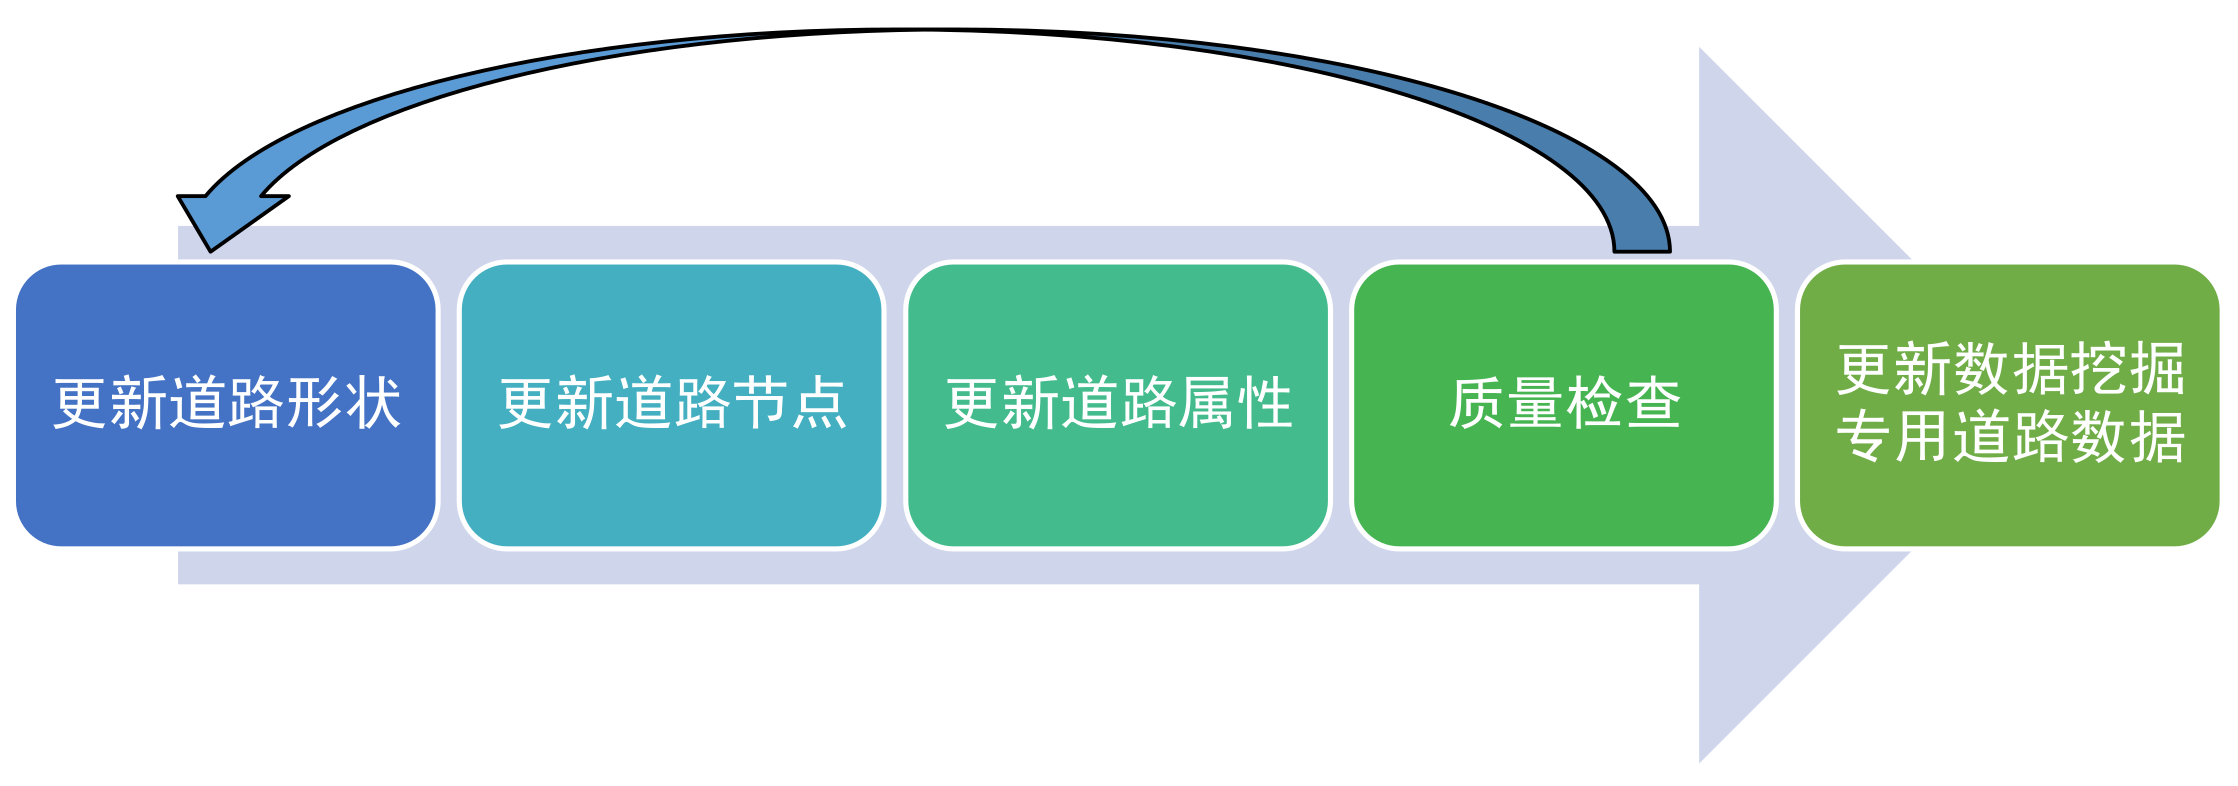
\includegraphics[width=\textwidth]{chp02_道路数据更新流程.png}
  \caption{道路数据更新流程\label{fig:道路数据更新流程} }
\end{figure}

\subsubsection{更新道路形状}
道路形状更新有三种情况:新增路段、删除路段和修改路段。

\smalltitle{新增路段}
新增路段在年度更新中出现的情况最多,主要工作是把年度新增的道路在
GIS 数据中进行更新,包括以下三种场景:

\begin{nbeae}
\item 在两个已有节点之间增加路段\\
\indenttext{在两条道路的交叉口之间新修道路时适用此情况。}

\indtentext{操作步骤:打开 ArcMap 的节点捕捉功能,先选择其中一个已有节点;然后
再根据信息中心底图数据的形状绘制新增路段,直至另一个已有节点;最后结束
形状编辑操作。}

\indenttext{如下图所示,在 16258 节点和 16362 节点之间新增路段。}

\begin{figure}[ht]
  \centering
  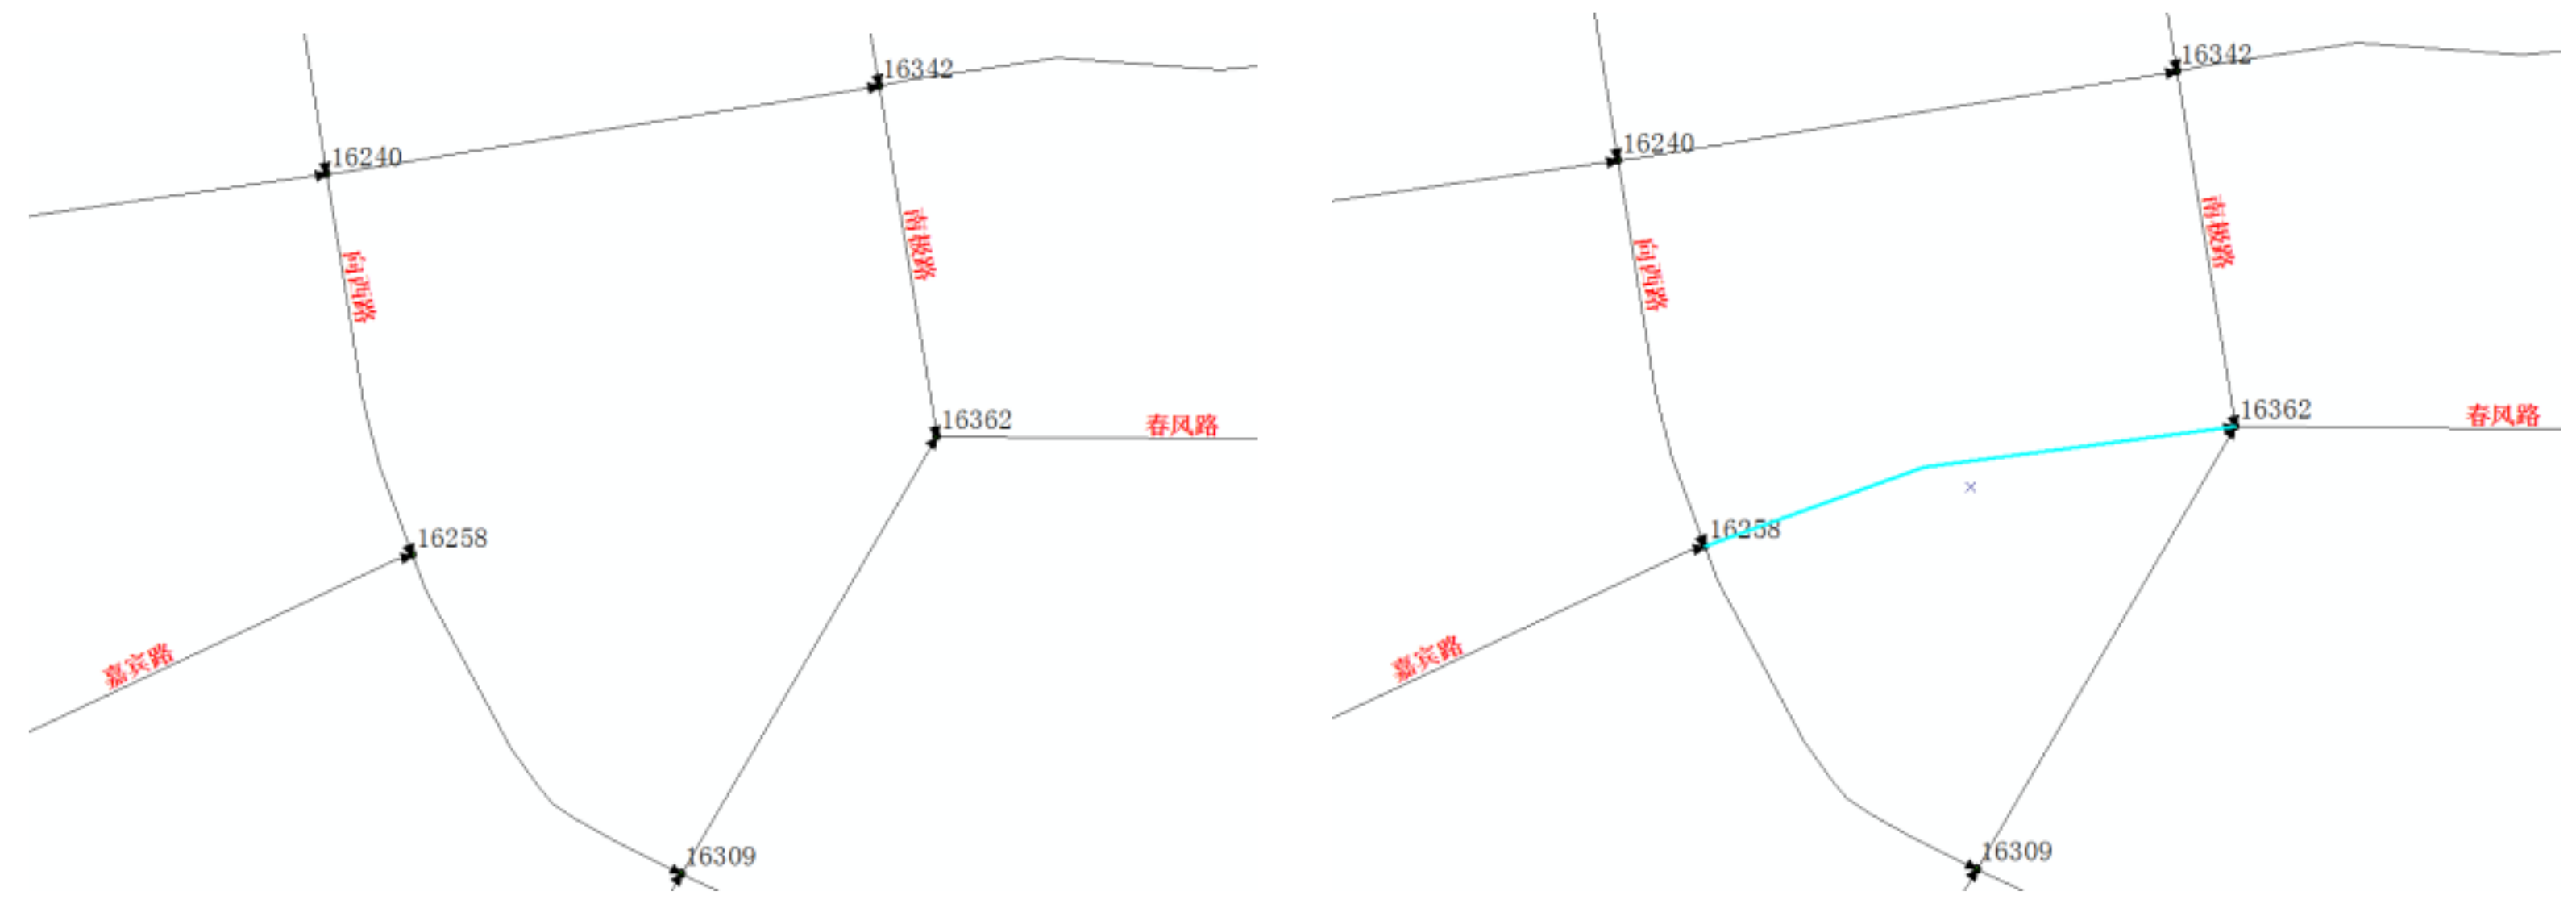
\includegraphics[width=\textwidth]{chp02_在已知两个节点之间增加路段.png}
  \caption{在已知两个节点之间增加路段\label{fig:在已知两个节点之间增加路段} }
\end{figure}

\item 在一个已有节点和一个新增节点之间增加路段\\
\indenttext{在一条道路的交叉口与另一条道路新增交叉口之间新修道路时适用此情况。}

\indenttext{操作步骤:首先根据信息中心底图数据的形状,将已有路段打断;然后在打
断的位置处新增一个节点,最后按照(a)的步骤在已有节点和新增节点绘制新增路段。}

\begin{figure}[ht]
  \centering
  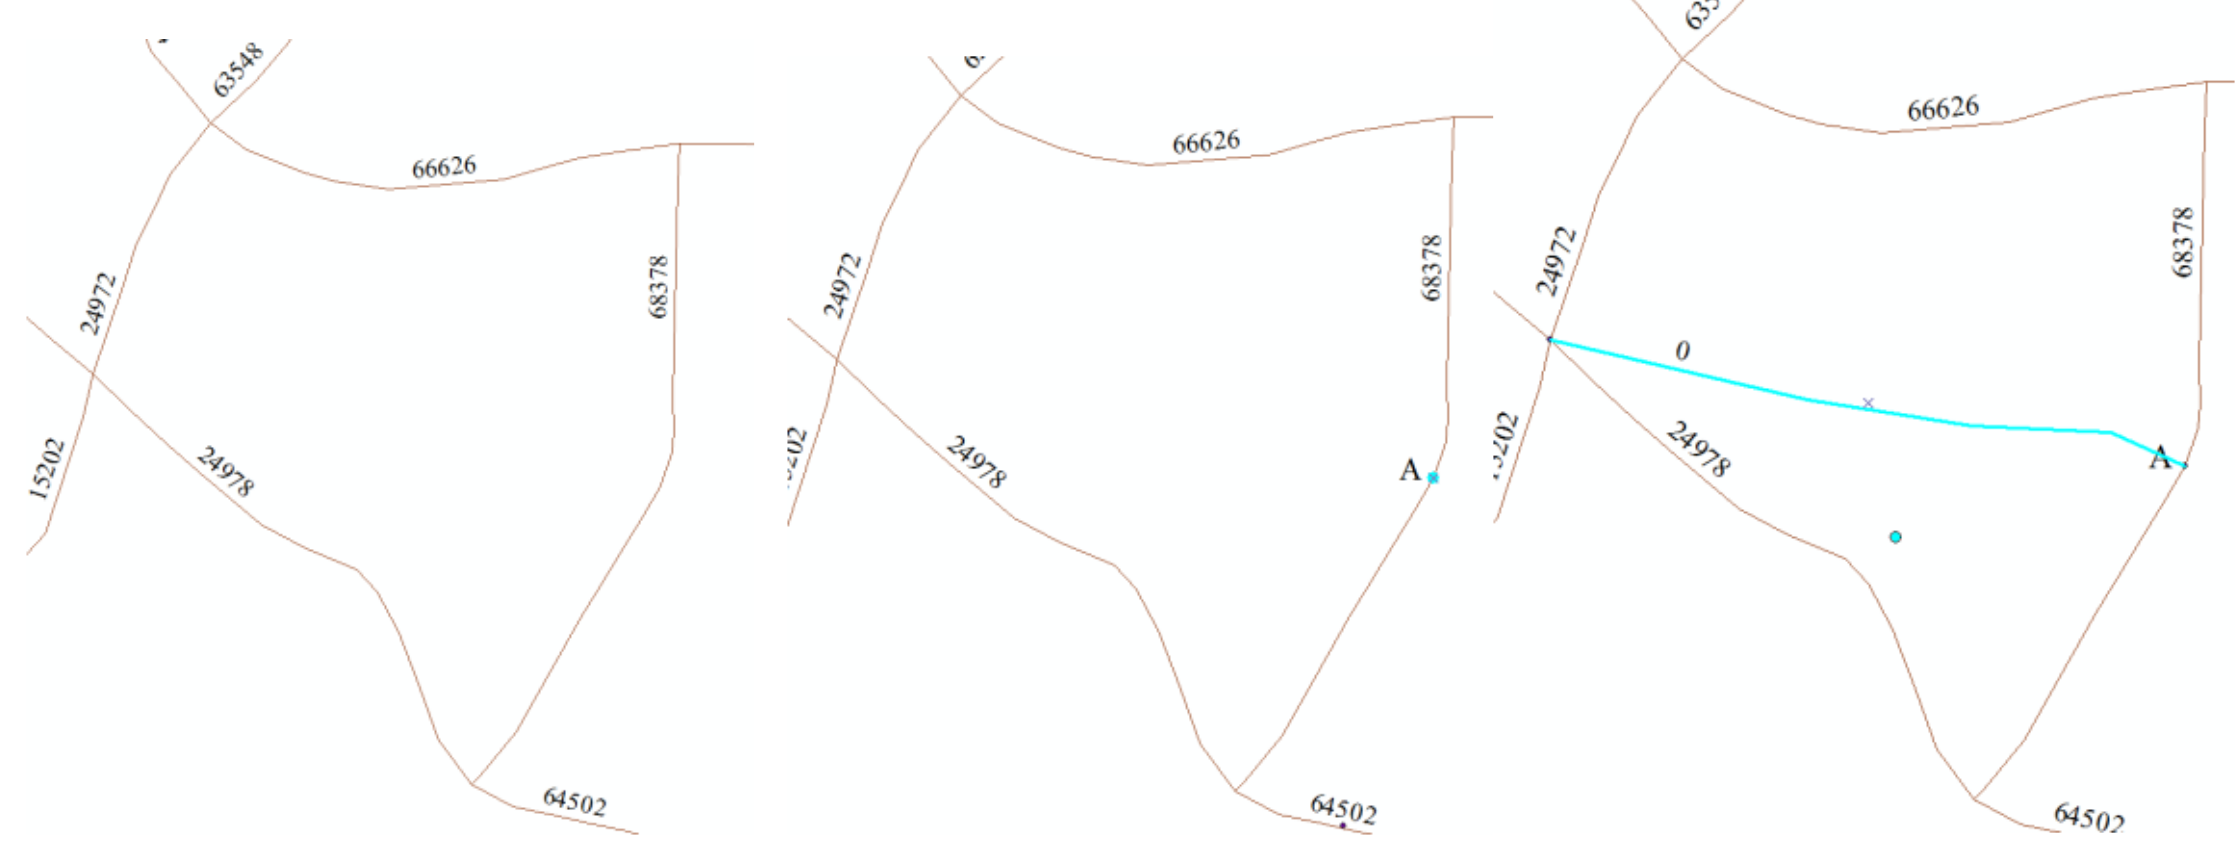
\includegraphics[width=\textwidth]{chp02_在一个已有节点和一个新增节点之间增加路段.png}
  \caption{在一个已有节点和一个新增节点之间增加路段\label{fig:在一个已有节点和一个新增节点之间增加路段} }
\end{figure}

\item 在两个新增节点之间增加路段\\
\indenttext{在两个新增节点之间增加路段的情况较少出现,适用于在两条道路都新增的交叉口之间新修道路的场景。
操作步骤与(1)类似,但是需要在两条道路上都先做打断和新增节点操作。}
\end{nbeae}

\smalltitle{删除路段}
删除路段用于原先绘制的道路错误、道路废弃等情况,一般较少出现。

操作步骤:首先选中需要删除的路段,然后点击删除指令,最后结束编辑。

\smalltitle{修改路段}
修改路段主要用于道路大致位置不变,即首尾节点不变的情况下,原绘制的
路段形状与实际情况存在较大差异时,需要对道路的形状进行修正。修改路段形
状对于道路原有的连接关系没有影响,不会影响交通仿真模型的运算结果,但是
会影响数据挖掘中 GPS 数据地图匹配的精度。

操作步骤:选择待修改路段,打开节点编辑功能,按照信息中心底图进行形
状修改,最后结束编辑。

\subsubsection{更新道路节点}
道路节点的更新主要是在道路形状发生改变的路段基础上,新增相应的道路
节点,用于表示道路交叉口;另外,还会对原有的道路节点进行删除和修改等修
复性工作。按照深圳市交通仿真系统(二期)的数据需求,在所有会发生行驶转
向的交叉口都需要有相应的节点数据,而其他情况的节点都不需要保存。

操作步骤:打开捕捉节点功能,按照实际的道路交叉口进行新增节点、删除
节点和修改节点的操作,最后结束编辑。

更新道路节点的工作需要特别注意是高架桥和隧道等区域,在这些区域由于
道路与道路是立体交叉的,并不会产生行驶转向,因此不能仅通过图形判断,必
须进行实地踏勘或者从卫星影像图中获得实际的转向信息。

\subsubsection{更新道路属性}
上述两个步骤完成了道路的基本形状:路段和节点的更新,但是道路是具有
特殊交通属性的线状实体,因此要在形状更新的基础上进一步更新道路的交通属
性信息,用于描述真实的道路。道路的属性更新工作可以和形状更新同步开展,
也可以在形状更新之后批量修改,所有的操作都由人工完成。

深圳市交通仿真系统(二期)中构建的路段图层 Roadlink 和节点图层
RodeNode 的属性信息如下。

\renewcommand{\arraystretch}{0.8}
\begin{longtable}[c] {|m{0.2\textwidth}|m{0.25\textwidth}|>{\centering\arraybackslash}m{0.1\textwidth}|
>{\baselineskip=14pt}m{0.32\textwidth}|} 
\caption{路段图层Roadlink属性信息\label{tbl:路段图层Roadlink属性信息}}
\hline
\multicolumn{1}{|c|}{\bfseries 属性名称} & \multicolumn{1}{c|}{\bfseries 含义} & 
  \multicolumn{1}{c|}{\bfseries 类型} & \multicolumn{1}{c|}{\bfseries 说明}\\\hline

NO & 唯一ID & Long & \\\hline
FNO & 起节点编号 & String & 最长5位,与RoadNode的WYID同 \\\hline
TNO & 终节点编号 & String & 最长5位,与RoadNode的WYID 同 \\\hline
FROM\_NAME & 起始道路名 & String & 本图层的DLMC字段 \\\hline
TO\_NAME & 终止道路名 & String & 本图层的DLMC字段 \\\hline
NAME & 道路名称 & String & 中文 \\\hline
CDS & 车道数 & String & F$\rightarrow$T方向车道数,数字\\\hline
LEN & 路段长度 & Float & 单位米\\\hline
LDKD & 路段宽度 & String & 单位米\\\hline
F\_T & 起节点向终节点方向 & String & 1:通行; 0:不通行\\\hline
T\_F & 终节点向起节点方向 & String & 1:通行; 0:不通行\\\hline
\multirow{7}{*}{DLDJ} & \multirow{7}{*}{道路等级} & \multirow{7}{*}{String} & 8:高速公路\\
& & & 7:快速路 \\
& & & 9:匝道 \\
& & & 6:主干道 \\
& & & 4:次干道 \\
& & & 2:支路 \\
& & & 99:小区道路\\\hline
SZXZQ & 所在行政区 & String & 行政区图层的WYID \\\hline
SZJTXQ & 所在交通小区 & String & 交通小区图层的WYID \\\hline
SZJD & 所在街道 & String & 街道图层的WYID \\\hline
SZZT & 所在组团 & String & 组团图层的WYID \\\hline
SZFDTZ & 所在法定图则 & String & 法定图则图层的WYID \\\hline
\end{longtable}

\renewcommand{\arraystretch}{0.8}
\begin{longtable}[c] {|m{0.2\textwidth}|m{0.25\textwidth}|>{\centering\arraybackslash}m{0.1\textwidth}|
>{\baselineskip=14pt}m{0.32\textwidth}|} 
\caption{节点图层Roadnode属性信息\label{tbl:节点图层Roadnode属性信息}}
\hline
\multicolumn{1}{|c|}{\bfseries 属性名称} & \multicolumn{1}{c|}{\bfseries 含义} & 
  \multicolumn{1}{c|}{\bfseries 类型} & \multicolumn{1}{c|}{\bfseries 说明}\\\hline

WYID & 唯一ID & String & 共 8 位,前两位为主要节点(Main Node)的首字母大写(MN),后六位与FID同,
不足以0代替,如:MN000017\\\hline
JDMC & 节点名称 & String & \\\hline
SZXZQ & 所在行政区 & String & 行政区图层的WYID \\\hline
SZJTXQ & 所在交通小区 & String & 交通小区图层的WYID \\\hline
SZJD & 所在街道 & String & 街道图层的WYID \\\hline
SZZT & 所在组团 & String & 组团图层的WYID \\\hline
SZFDTZ & 所在法定图则 & String & 法定图则图层的WYID \\\hline
ZBX & 坐标X & Double & \\\hline
ZBY & 坐标Y & Double & \\\hline
\end{longtable}

路段图层包含的属性信息非常多,其中必须要更新的为路段唯一 ID 字段,
起止节点编号字段,路段长度字段,起节点向终节点方向和终节点向起节点方向
字段,道路等级字段,所在行政区、所在交通小区、所在街道、所在组团、所在
法定图则、所属吸引点字段。

其中,新增加路段的 NO 值,在原有最大 NO 值的基础上增加 1 或 2,如为
单行线,则为 1,如为双行线,则为 2;如果删除路段,原有的 NO 值不再使用,
修改路段不需要修改原有 NO 值。路段长度、起节点向终节点方向和终节点向起
节点方向、所在行政区、所在交通小区、所在街道、所在组团、所在法定图则、
所属吸引点字段可以在形状更新完成后通过 ArcGIS 自带的数据处理工具自动化
辅助更新。

节点图层必须要更新的字段是唯一 ID 和坐标 X、坐标 Y。其中,新增加节
点的 WYID 值,在原有最大 WYID 值的基础上增加 1;坐标 X 和坐标 Y 可以在
形状更新完成后通过 ArcGIS 自带的数据处理工具自动化辅助更新。

\subsubsection{质量检查}
由于上述的操作主要由人工完成,所以在操作过程中难免会出现一些错误,
因此需要通过预设的一些规则自动筛选出可能出现错误的地方,然后再通过人工
判断确定错误的位置,最后按照上述形状和属性更新的步骤来修复错误。为了保
证数据的质量,质量检查工作同时由多人配合完成。

数据质量检查包括操作过程中的日志记录和后期的自动化检查两部分。其中
日志记录是今年新引入的一种工作模式,其原理是在每一步操作中记录操作内容
和操作时间,目的是为了能够在后期检查中发现错误操作时能够进行有效的回退
操作,减少人工排查的工作量并提高修复精度。

自动化检查部分包括:路段 ID 的唯一性检查、小路段的检测与修复、断头路的检测与修复、
相连相同路段的检测与修复以及道路立体交叉处的连接关系修复。

\smalltitle{路段 ID 的唯一性检查}
路段的 ID 是后续数据挖掘和数据查询的重要条件,如果在人工作业中出现
了重复 ID,则会导致后续挖掘和数据查询的错误结果,因此需要通过程序自动
化检查路段 ID 是否出现重复。

\smalltitle{小路段的检测与修复}
小路段是指路段长度小于一定阈值的路段。小路段的存在大大增加了系统负
荷,降低了系统执行效率。因此,本项目以 50 米为阈值,对全路网进行检测,
并人工编辑修复 50 米以下路段。

\begin{figure}[ht]
  \centering
  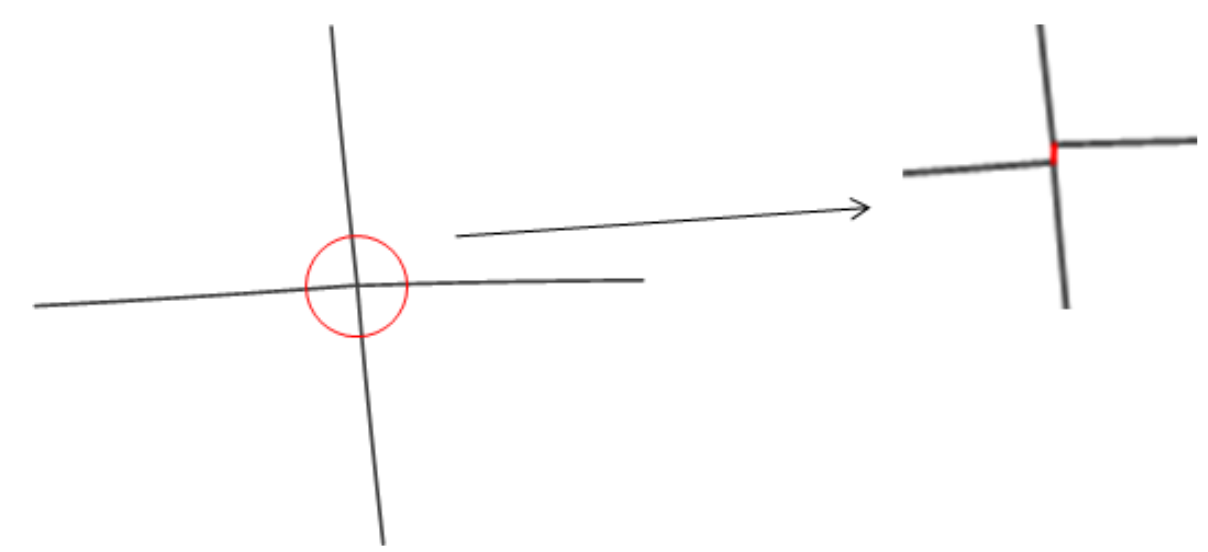
\includegraphics[width=0.6\textwidth]{chp02_小路段的检测与修复.png}
  \caption{小路段的检测与修复\label{fig:小路段的检测与修复}}
\end{figure}

\smalltitle{断头路的检测与修复}
断头路是指路段到了终点后,没有后续相连的道路与之连接。断头路分为正
常断头路和非正常断头路。非正常断头路事实上是拓扑逻辑存在问题的区域,因
此必须予以消除。

\begin{figure}[ht]
  \centering
  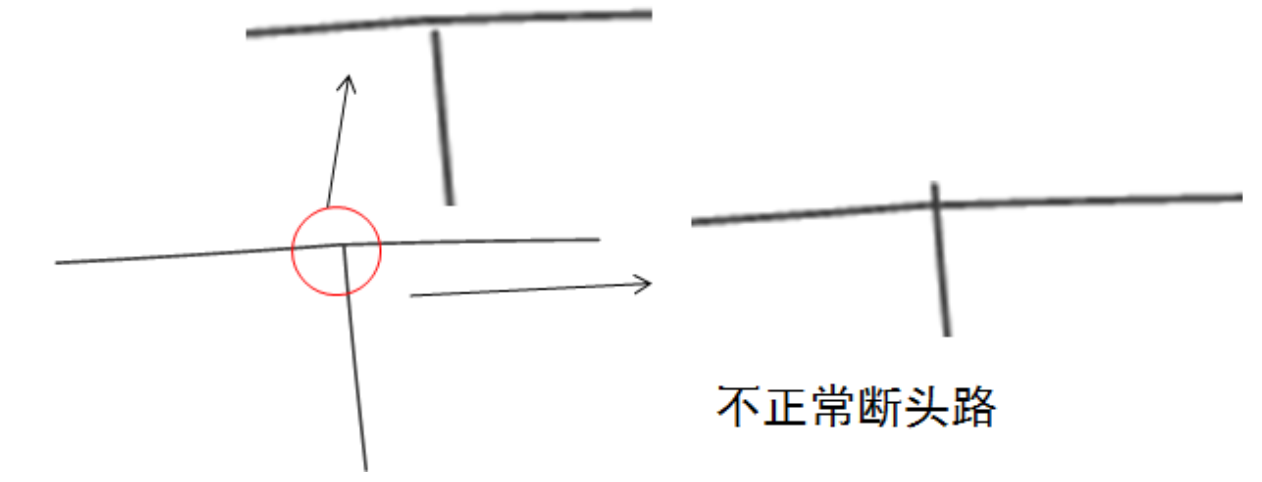
\includegraphics[width=0.6\textwidth]{chp02_断头路的检测与修复.png}
  \caption{断头路的检测与修复\label{fig:断头路的检测与修复}}
\end{figure}

\smalltitle{相连相同路段的检测与修复}
相连相同路段是指道路名称(DLMC)、车道数(CDS)、道路等级(DLDJ)、
分割类型(CGLX)等四个关键属性完全一致的道路,这种类型的道路事实上可
以进行合并管理

\begin{figure}[!ht]
  \centering
  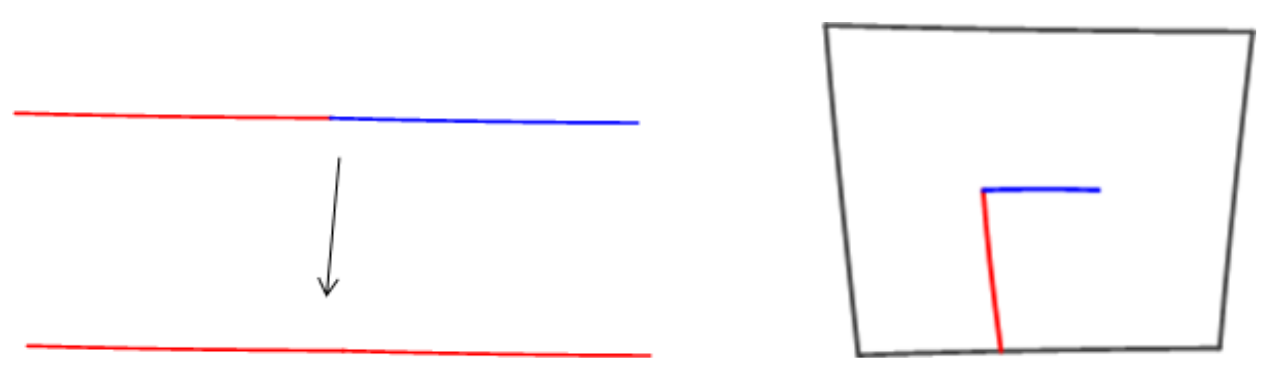
\includegraphics[width=0.6\textwidth]{chp02_相连相同路段的检测与修复.png}
  \caption{相连相同路段的检测与修复\label{fig:相连相同路段的检测与修复}}
\end{figure}

\smalltitle{道路立体交叉处的连接关系修复}
对于匝道、立交桥、隧道等立体交叉位置,采用卫星影像辅助人工判断道路的实际连接关系。

\begin{figure}[!ht]
  \centering
  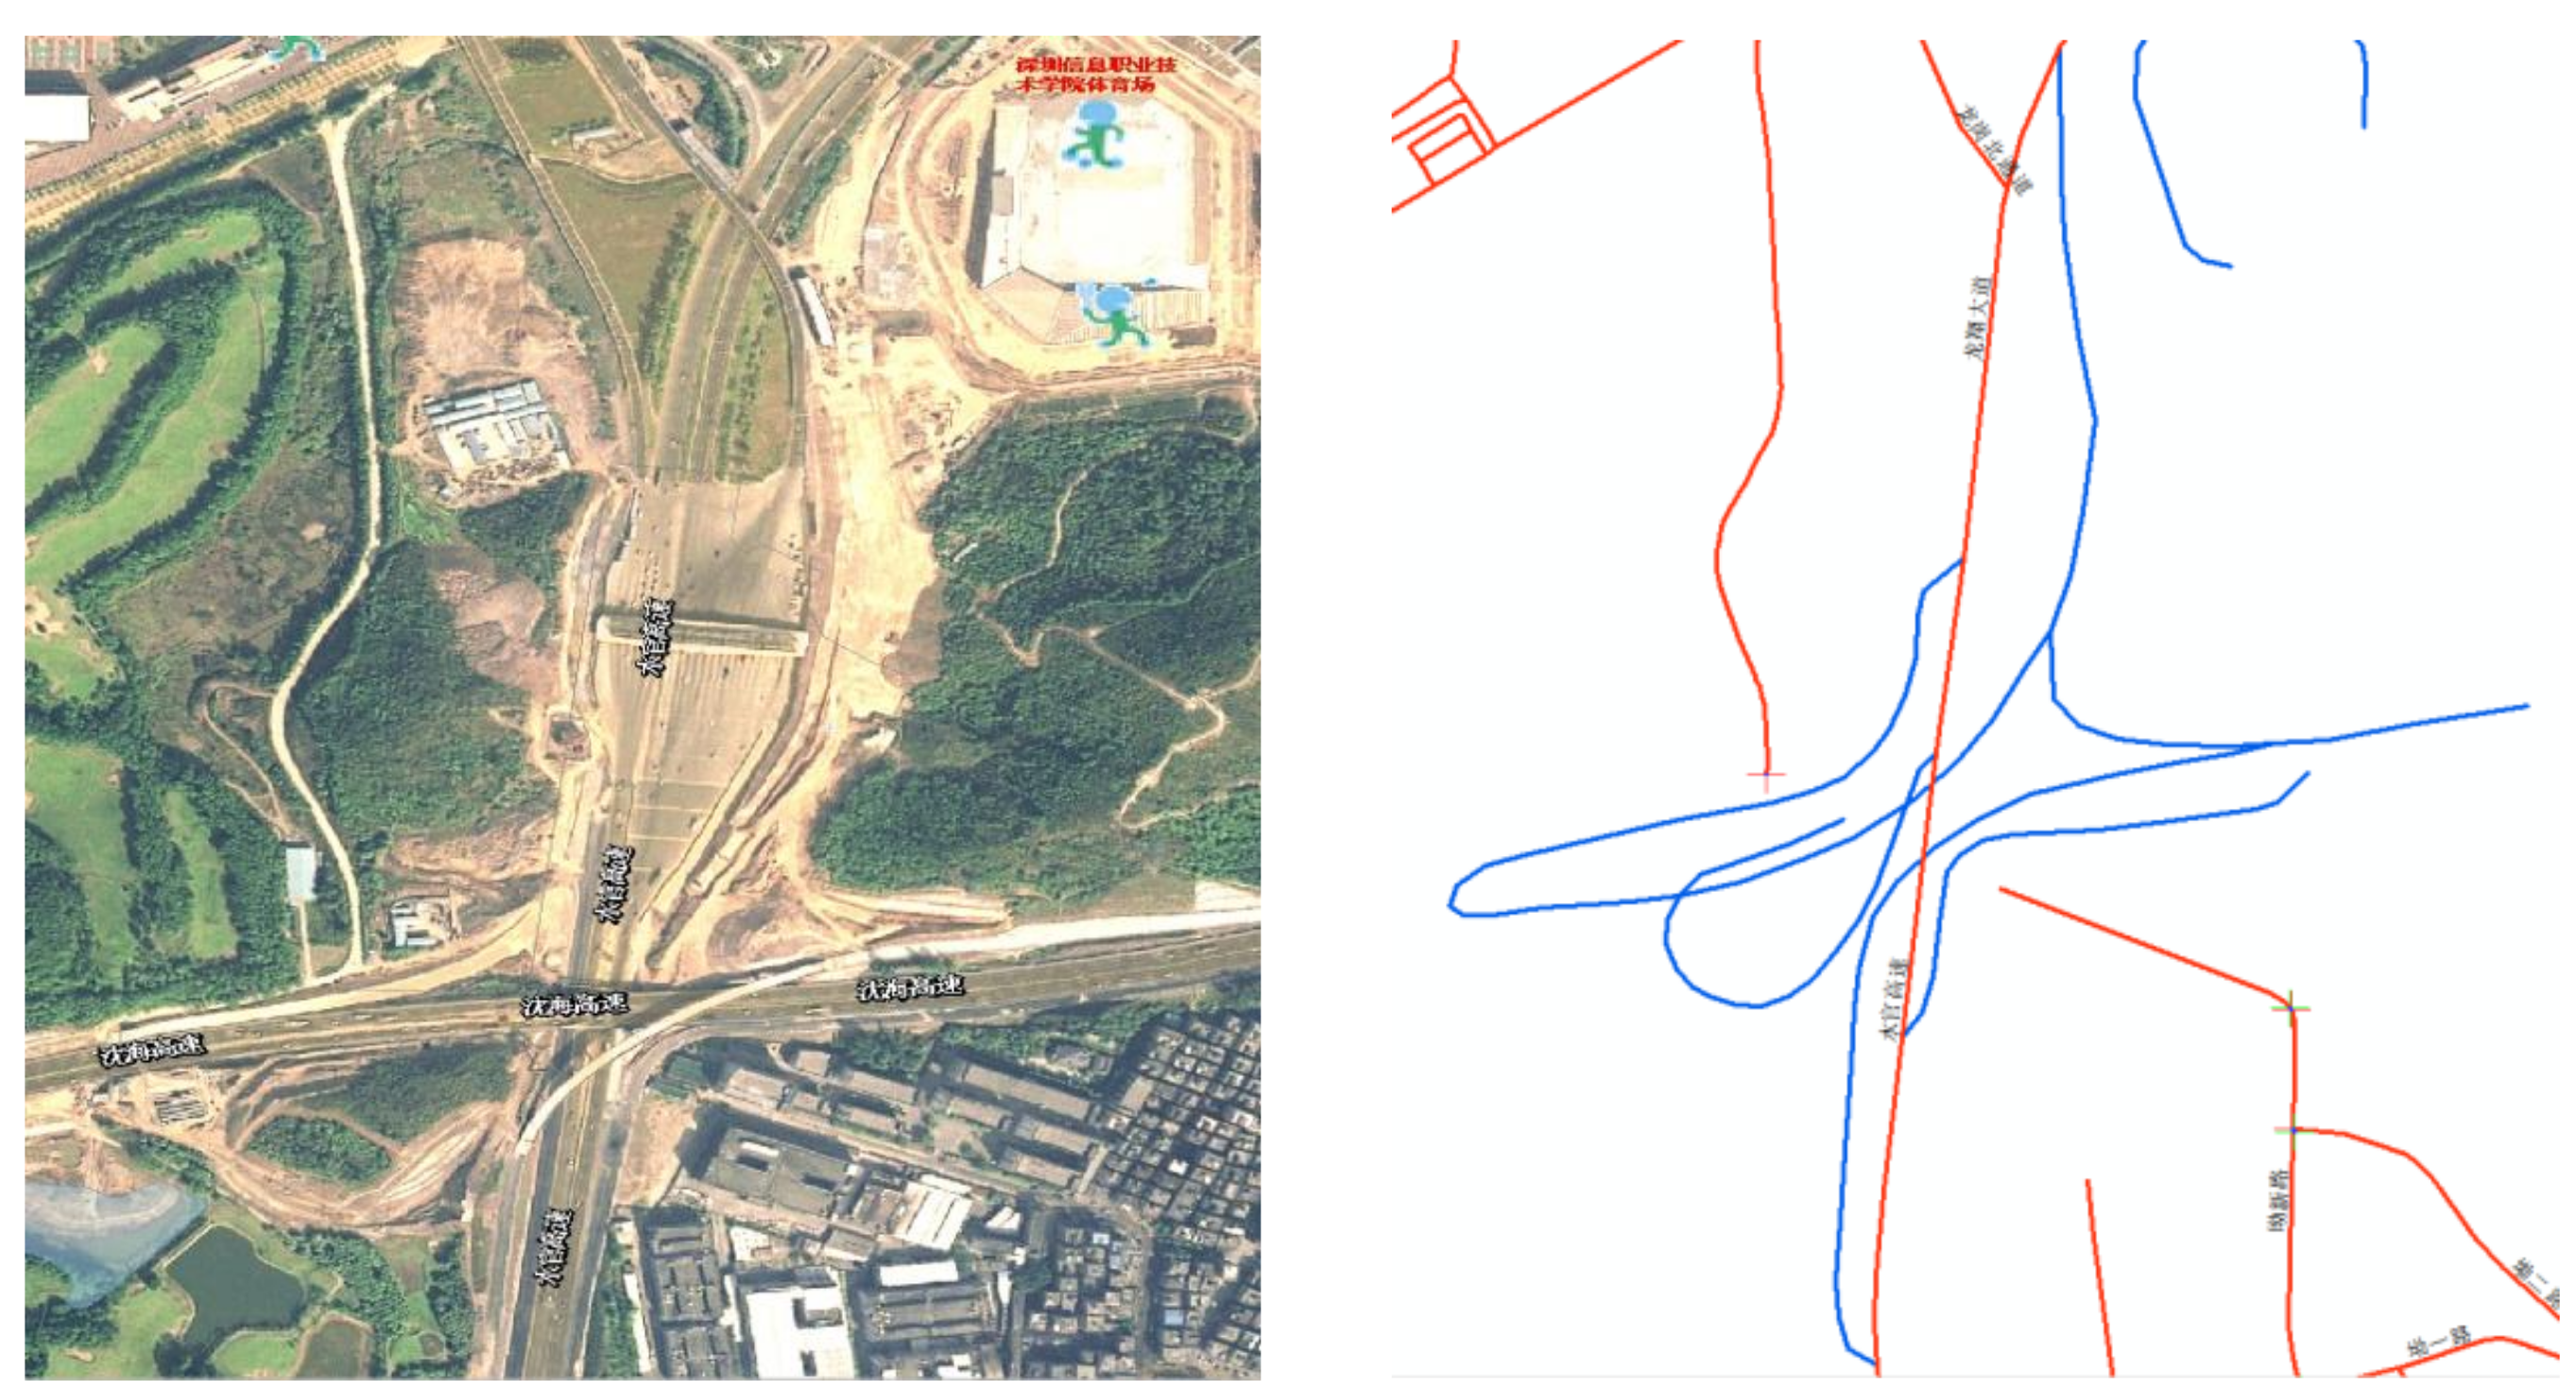
\includegraphics[width=0.8\textwidth]{chp02_道路立体交叉处的连接关系修复.png}
  \caption{道路立体交叉处的连接关系修复\label{fig:道路立体交叉处的连接关系修复}}
\end{figure}

\subsubsection{更新数据挖掘专用道路数据}
经过前面的道路更新工作后,道路的形状和属性数据都已经更新至\pyear 年,
可以用于后续的数据查询系统和交通模型系统更新。 但是, 数据挖掘中的路段车
速计算需要对原有的道路数据进行进一步的处理,使其符合数据挖掘系统的输入
需要。 经过处理后的数据包括: 数据挖掘专用路段图层 GIS 数据、 地图索引文
件和路段编号与小区编号对应文件。 具体处理操作如下:

\smalltitle{坐标转换}
但是, 由于数据挖掘系统中的路段车速计算需要将车辆 GPS 数据与道路数
据进行地图匹配, 而上述所有操作都是在深圳本地坐标系下, 和 GPS 数据的
WGS84 坐标不匹配。 因此, 需要首先通过 ArcGIS 空间纠正工具将原有道路形状
纠正到 WGS84 坐标系下。

\smalltitle{路段图层属性转换}
另外, 深圳市交通仿真系统(二期)中采用的路段车速计算程序对道路网络
的输入有一套自定义的规则,与表 4 中的字段有差别, 所以需要对 RoadLink 图
层的字段进行转换处理,使其符合路段车速计算程序的输入要求。 下表为路段车
速计算程序输入的路段图层字段要求, 以及与表\ref{tbl:路段图层Roadlink属性信息}的转换关系。

\renewcommand{\arraystretch}{0.8}
\begin{longtable}[c] {|m{0.15\textwidth}|C{0.1\textwidth}|C{0.15\textwidth}|C{0.25\textwidth}|m{0.2\textwidth}|} 
\caption{数据挖掘专用道路数据结构\label{tbl:数据挖掘专用道路数据结构}}
\hline
\multicolumn{1}{|c|}{\bfseries 字段名} & \multicolumn{1}{c|}{\bfseries 类型} & 
  \multicolumn{1}{c|}{\bfseries 含义} & \multicolumn{1}{c|}{\bfseries 取值范围} &
\multicolumn{1}{C{0.2\textwidth}|}{\bfseries 与Roadlink图层对应关系}\\\hline

EDGEID & Int(10) & 路段编号 & & NO \\\hline
FJCID & Int(10) & 起点编号 & & FNO \\\hline
TJCID & Int(10) & 终点编号 & & TNO \\\hline
LENGTH & Float & 路段长度 & 单位米 & LEN \\\hline
BYNAMEC & Char(20) & 道路名称 & & NAME \\\hline
\multirow{4}{*}{DF} & \multirow{4}{*}{Int(2)} & \multirow{4}{*}{交通流方向} & 1:双向可通行 & \multirow{4}{*}{F\_T,T\_F}\\
 & & & 2:与矢量方向相同 &\\
 & & & 3:与矢量方向相反 &\\
 & & & 4:双向不通行 & \\ \hline
\multirow{8}{*}{NR} & \multirow{8}{*}{Int(2)} & \multirow{8}{*}{管理等级} & 1:高速路 &  \multirow{8}{*}{DLDJ} \\
& & & 2:国道 & \\
& & & 3:快速路 & \\
& & & 4:省道 & \\
& & & 5:主干道 & \\
& & & 6:次干道 & \\
& & & 7:支路 & \\
& & & 8:支路以下 & \\\hline 
\end{longtable}

\subsection{公交数据更新}
公交数据更新的技术方法是:基于交委发布的现状公交站点名称数据,并结
合商业地图中的现状公交站点位置数据,以深圳市交通仿真系统(二期)原有的
公交站点图层(BusStop)为基础,采用半自动化方式进行新增和修改操作;然
后再通过专门开发的程序,按照站点位置和线路站点顺序,重新生成公交线路,
直接更换原有数据。

更新的流程包括更新公交站点位置和名称、公交网检查、生成公交线路和更
新线路和站点属性四个环节。

\begin{figure}[ht]
  \centering
  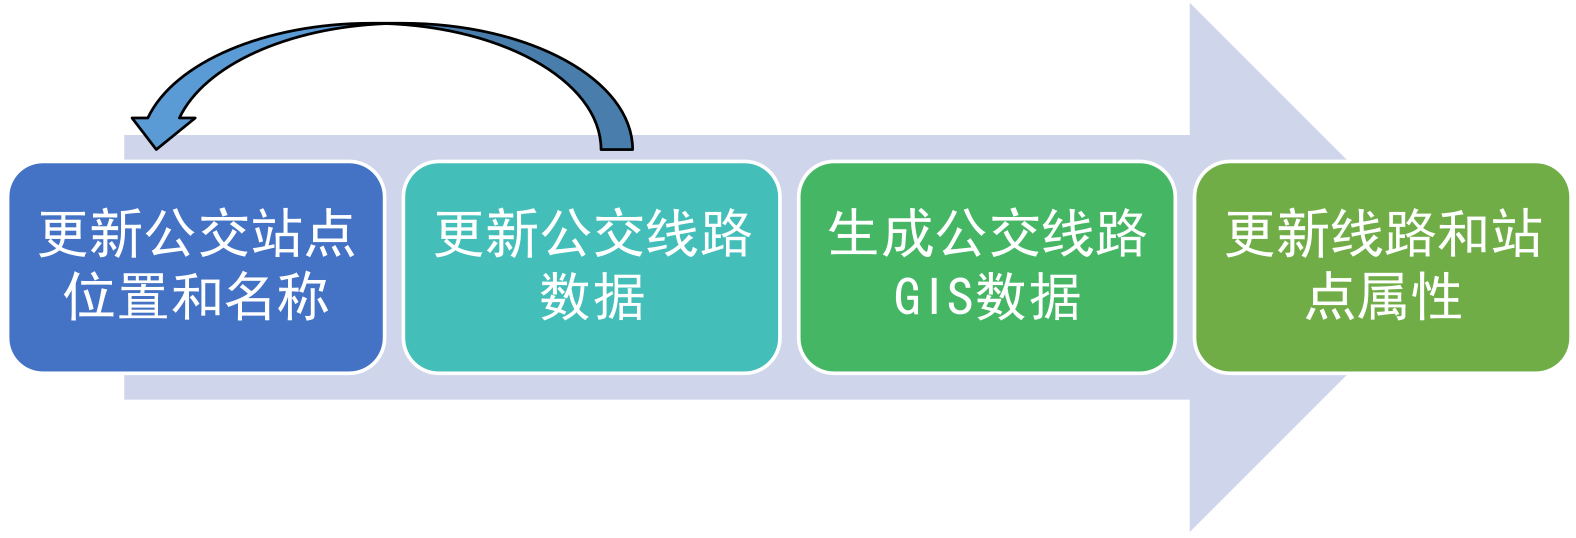
\includegraphics[width=\textwidth]{chp02_公交数据更新流程.png}
  \caption{公交数据更新流程\label{fig:公交数据更新流程} }
\end{figure}

\subsubsection{更新公交站点位置和名称} \label{subsubsec:更新公交站点位置和名称}
深圳市交委每个月都会在官方网站上提供最新的公交线路和途经站点文件,
文件主要包括线路编号、起点站、终点站、上行途经站点、下行途经站点、上行
途经道路和下行途经道路字段。

但是,文件中途经站点只有中文名称,并没有位置数据。因此,首先通过程
序在文件中自动化搜索出在原有文件中没有出现过的站点名称,然后再通过商业
地图,通过人工方式依次在 BusStop 图层中新增公交站点位置。其中,在进行新
增公交站点的操作过程中,也同时对 WYID 字段进行更新。WYID 字段是按
“BS”+五位数字规则定义的,新增的公交站点在原有最大五位数字的基础上增
加 1。

\begin{figure}[!ht]
  \centering
  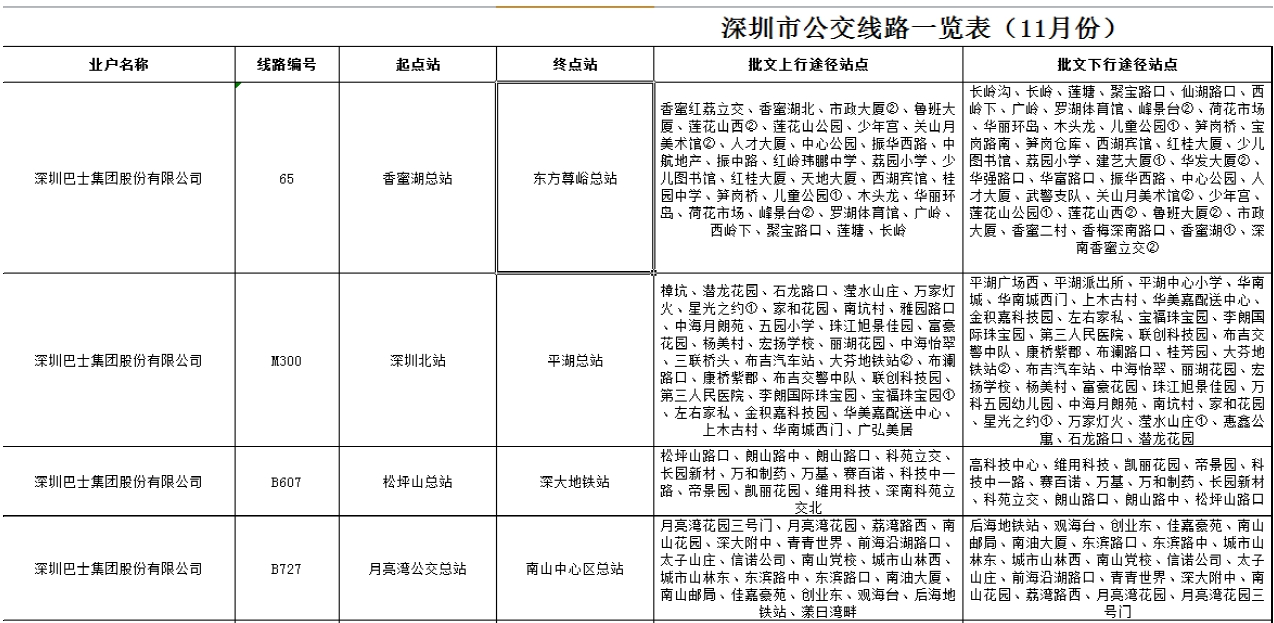
\includegraphics[width=\textwidth]{chp02_深圳市交委官方网站提供的公交线路一览表.jpg}
  \caption{深圳市交委官方网站提供的公交线路一览表\label{fig:深圳市交委官方网站提供的公交线路一览表} }
\end{figure}

\begin{figure}[!ht]
  \centering
  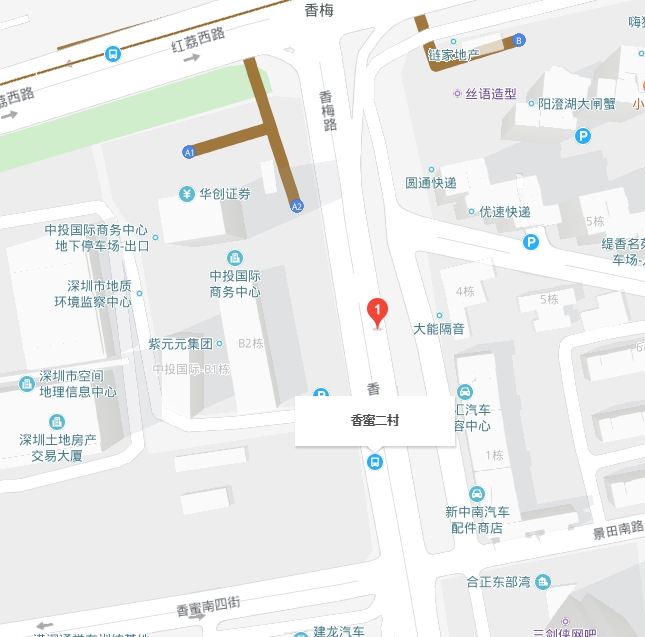
\includegraphics[width=0.5\textwidth]{chp02_通过商业地图确定新增公交站点位置.jpg}
  \caption{通过商业地图确定新增公交站点位置\label{fig:通过商业地图确定新增公交站点位置} }
\end{figure}

更新后的公交站点图层导出为一个文本文件,包含公交站点唯一 ID (WYID)、
站点名称(ZDMC)、站点 X 坐标(ZBX)和站点 Y 坐标(ZBY)四个字段。其中需要特别注意的是:

\begin{cit}
\item WYID 字段不能出现重复,且每条记录非空
\item ZDMC 字段建议删除“?”等非法字符
\item ZBX、ZBY 为深圳本地坐标系,且每条记录非空
\item 合法符号转换,建议将合法的符号全部转换为全角字符
\end{cit}

\subsubsection{更新公交线路数据} \label{subsubsec:更新公交线路数据}
根据\fref{fig:深圳市交委官方网站提供的公交线路一览表}的公交线路一览表以及上节生成的公交站点文本文件,对公交
线路途经站点按照中文名称与编号的对应关系进行标准化,生成公交线路站点顺
序描述表,包括线路和途经站点两个字段,中间用英文符号 “,” 分隔;途经站点
之间用中文符号“、”分隔。这个步骤可以编写程序自动化完成。

\begin{figure}[ht]
  \centering
  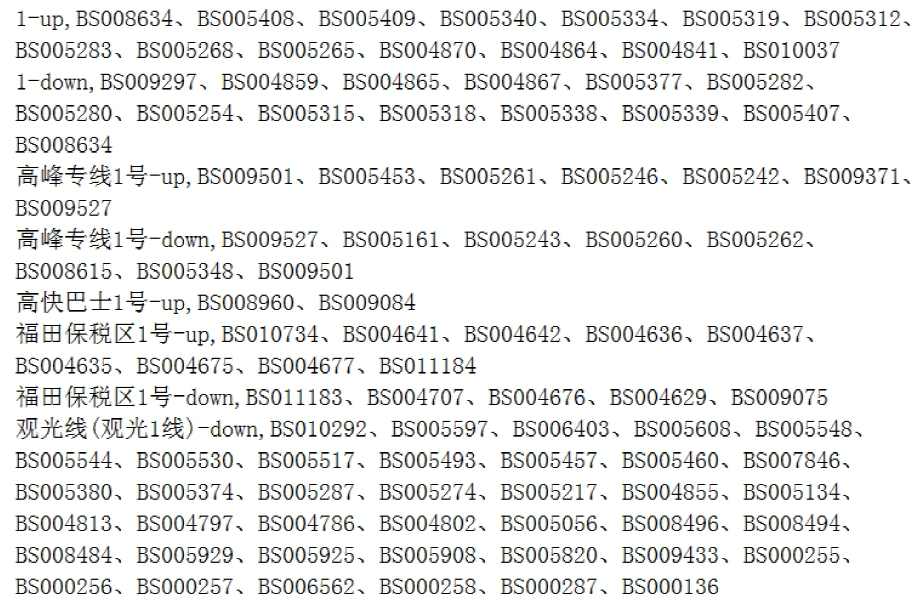
\includegraphics[width=0.7\textwidth]{chp02_公交线路站点顺序描述表.jpg}
  \caption{公交线路站点顺序描述表\label{fig:公交线路站点顺序描述表} }
\end{figure}

另外,还需要按照线路途经的每个站点一条记录的形式生成公交线路站点描
述表文件,包括线路 ID(RouteID)、公交站点 ID(StopID)、公交站点名称
(StopName)和公交站点坐标(X 和 Y)五个字段,中间以英文符号“,”分隔。

\begin{figure}[ht]
  \centering
  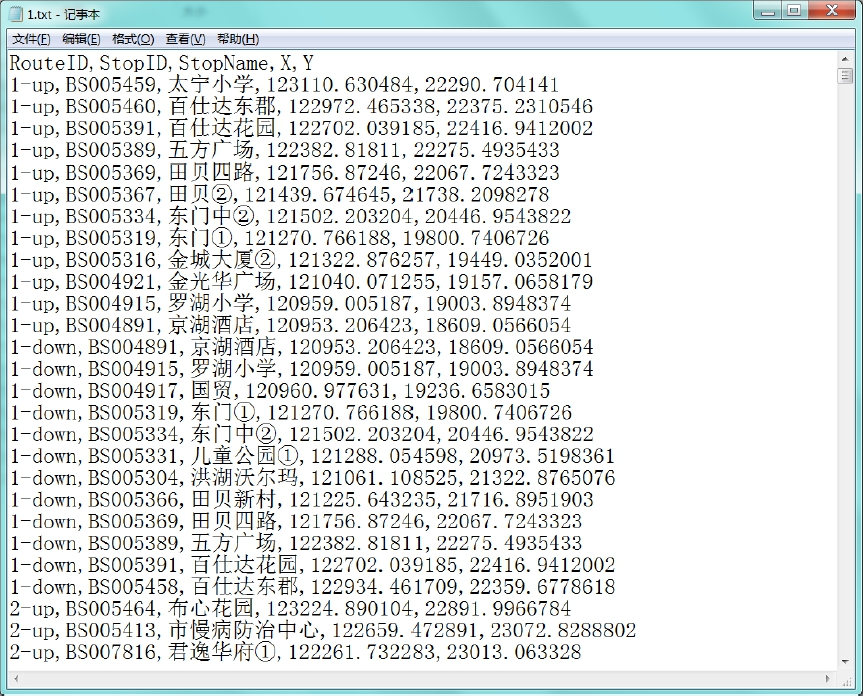
\includegraphics[width=0.7\textwidth]{chp02_公交线路站点顺序表.jpg}
  \caption{公交线路站点顺序表\label{fig:公交线路站点顺序表} }
\end{figure}

\subsubsection{生成公交线路 GIS 数据}
按照深圳市交通仿真系统(二期)的设计,公交线路 GIS 数据包括公交线
路图层(BusRoute)和公交线段图层(BusLink)。公交线路图层是按照每条公交
线路一个完整 polyline 实体进行存储的,而公交线段图层是对公交线路图层在每
个公交站点处打断生成的,一条公交线路中的每两个连续公交站点之间形成一个
polyline 实体。因此,首先生成公交线路图层,再生成公交线段图层。

\smalltitle{生成公交线路图层}
生成公交线路图层工作利用 ArcGIS Network Analysis 模块进行自动化完成。
具体步骤如下:

\begin{nbeae}
\item 将上节得到的公交线路站点描述表文件导入 ArcMap,使用“add
xy data”功能转换为 shapefile 点文件,坐标为 ZBX 和 ZBY;
\item 在 ArcCatalog 中,选择更新后的路段 GIS 文件 RoadLink,选择“Create Network
dataset”功能创建路网的网络数据集;
\item 在 ArcMap 中加载上一步中创建的网络数据集和(a)中的公交线路站点描述表图层,
打开 Network Analysis 模块,新增一个线路工程(add new route);
\item 采用 ArcToolbox$\rightarrow$Network analysis 工具$\rightarrow$添加位置功能,输入相应的数据;
其中,“输入网络分析图层”中输入(b)中创建的网络数据集,“子图层”输入(a)
中的公交线路站点描述表图层,“字段映射”的 RouteName 输入公交线路站点描述表图层中的线路编号字段 RouteID;
\begin{figure}[!htbp]
  \centering
  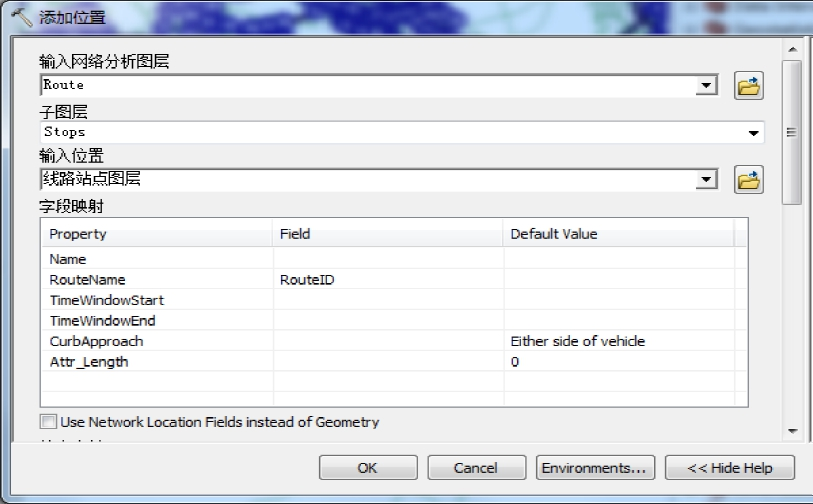
\includegraphics[width=0.7\textwidth]{chp02_公交线路站点描述表图层设置.jpg}
  \caption{公交线路站点描述表图层设置\label{fig:公交线路站点描述表图层设置} }
\end{figure}
\item 最后,使用 Network Analysis 模块中的 Solve 功能,自动生成线路。
\end{nbeae}

生成后的公交线路图层命名为 BusRoute。需要特别注意的是,BusRoute 图
层的唯一 ID 字段需要和深圳市交通仿真系统(二期)中使用的 BusRoute 图层的
唯一 ID 字段,根据线路名称字段进行连接操作(join),保证唯一 ID 在不同年
份的连续性和唯一性,使得在公交线路相关指标历史查询的正确性;当线路唯一
ID 无法与原有数据 join 时(无法 join 说明此线路为 2017 年新增线路),唯一 ID
按照最大 ID 值增加 1 来取值。

\smalltitle{生成公交线段图层}
由上述公交线路图层生成公交线段图层的工作由基于 ArcMap 组件开发的程
序自动完成,程序的主界面如下:
\begin{figure}[!htbp]
  \centering
  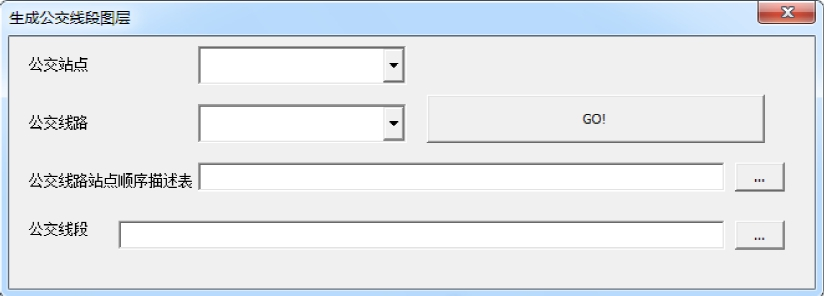
\includegraphics[width=0.7\textwidth]{chp02_生成公交线段图层程序界面.jpg}
  \caption{生成公交线段图层程序界面\label{fig:生成公交线段图层程序界面} }
\end{figure}

操作步骤如下:
\begin{nbeae}
\item “公交站点”输入\ref{subsubsec:更新公交站点位置和名称}节更新后的公交站点图层 BusStop;
\item “公交线路”输入\ref{subsubsec:更新公交线路数据}节生成的公交线路图层 BusRoute;
\item “公交线路站点顺序描述表”输入 2.2.3.2 节生成的公交线路站点顺序描述表;
\item “公交线段”输入需要导出公交线段图层的路径位置;
\item 点击“GO!”按钮进行运算,运算结束后会有对话框提示。
\end{nbeae}

生成后的公交线路图层命名为 BusLink。另外,运算程序不仅会自动打断并
生成公交线段,而且会在运算过程中将 BusRoute 图层的起止公交站点编号字段
(QDZH 和 ZDZH)自动更新。

\subsubsection{更新线路和站点属性}
上述几节的工作生成了公交站点图层 BusStop、公交线路图层 BusRoute 和公
交线段图层 BusLink 的 GIS 图形数据以及部分属性数据,本节需要继续对三个图
层的剩余属性数据进行补全。

\smalltitle{公交站点(BusStop)图层属性更新}
BusStop 图层的属性信息如表\ref{tbl:公交站点图层属性数据结构}所示。

\renewcommand{\arraystretch}{0.8}
\begin{longtable}[c] {|m{0.1\textwidth}|C{0.2\textwidth}|C{0.15\textwidth}|m{0.45\textwidth}|} 
\caption{公交站点图层BusStop属性数据结构\label{tbl:公交站点图层属性数据结构}}
\hline
\multicolumn{1}{|c|}{\bfseries 属性名称} & \multicolumn{1}{c|}{\bfseries 含义} & 
  \multicolumn{1}{c|}{\bfseries 类型} & \multicolumn{1}{c|}{\bfseries 说明}\\\hline

WYID & 唯一ID & String & BS+5位数字,例如BS00001\\\hline
ZDMC & 站点名称 & String & \\\hline
ZBX & 坐标 X & Double & \\\hline
ZBY & 坐标 Y & Double & \\\hline
SZXZQ & 所在行政区 & String & 行政区图层的WYID \\\hline
SZJTXQ & 所在交通小区 & String & 交通小区图层的WYID \\\hline
SZJD & 所在街道 & String & 街道图层的WYID \\\hline
SZZT & 所在组团 & String & 组团图层的WYID \\\hline
SZFDTZ & 所在法定图则 & String & 法定图则图层的WYID \\\hline
SZLDBH & 所在路段编号 & String & 即路段图层RoadLink的NO 字段 \\\hline
GNGW & 关内关外 & String & 1:关内; 2:关外 \\\hline
SSXYD & 所属吸引点 & String & \\\hline
\end{longtable}

其中, 唯一 ID( WYID)、站点名称( ZDMC)、坐标( ZBX 和 ZBY) 字段
在\ref{subsubsec:更新公交站点位置和名称}节的更新工作中已经完成,剩余的所在行政区、所在交通小区、所在
街道、所在组团、所在法定图则、所在路段编号、关内关外、所属吸引点字段可
以通过将 BusStop 图层与相应图层进行简单的空间关系判断来补全,全部操作都
使用 ArcMap 的空间连接功能完成。

\smalltitle{公交线路( BusRoute)图层属性更新}
BusRoute 图层的属性信息如表\ref{tbl:公交线路图层属性数据结构}所示。

\renewcommand{\arraystretch}{0.8}
\begin{longtable}[c] {|m{0.1\textwidth}|C{0.2\textwidth}|C{0.15\textwidth}|m{0.45\textwidth}|} 
\caption{公交线路图层BusRoute属性数据结构\label{tbl:公交线路图层属性数据结构}}
\hline
\multicolumn{1}{|c|}{\bfseries 属性名称} & \multicolumn{1}{c|}{\bfseries 含义} & 
  \multicolumn{1}{c|}{\bfseries 类型} & \multicolumn{1}{c|}{\bfseries 说明}\\\hline

ID & 唯一ID & String & BR+5位数字,例如BR00001\\\hline
NAME & 线路名称 & String & 由GJXLMC和上下行关键字组成,如1-up表示1路上行 \\\hline
GJXLMC & 公交线路名称 & String & 如M241, 115 \\\hline
SXX & 上下行 & String & 0:上行;1:下行 \\\hline
XLCD & 线路长度 & Double & 单位米\\\hline
YXGS & 运行公司 & String & \\\hline
QDZM & 起点站名 & String & 与BusStop图层的ZDMC字段相同 \\\hline
QDZH & 起点站号 & String & 与BusStop图层的WYID字段相同 \\\hline
ZDZM & 终点站名 & String & 与BusStop图层的ZDMC字段相同根据QDZM和ZDZM就可以区分上下行 \\\hline
ZDZH & 终点站号 & String & 与BusStop图层的WYID字段相同根据QDZH和ZDZH就可以区分上下行 \\\hline
YTCZ & 沿途车站 & String & 首末车站的中间车站的WYID,按顺序输入,由逗号分隔 \\\hline
GNGW & 关内关外 & Integer & 1:全部关内;2:全部关外;3:关内关外 \\\hline
\end{longtable}

其中, 唯一 ID( WYID)、线路名称( NAME) 字段、起点站号( QDZH)
和终点站号( ZDZH) 字段在\ref{subsubsec:更新公交线路数据}节的更新工作中已经完成;公交线路名称
( GJXLMC)字段和上下行( SXX)字段可以根据线路名称字段进行简单的字符
分隔处理自动化获得;线路长度( XLCD) 字段在图形编辑完成后可以由 ArcMap
自动计算获得; 起点站名( QDZM)和终点站名( ZDZM) 字段可以采用 ArcMap
中的连接功能( join), 按照起点站号( QDZH) 和终点站号( ZDZH) 字段和公
交线路站点描述表中的公交站点编号和公交站点名称对应关系自动补全; 关内外
( GNGW) 字段可以通过将 BusRoute 图层与关内外区域图层进行简单的空间关
系判断来补全;运行公司 ( YXGS)字段,可以根据实际信息补全;沿途车站( YTCZ)
字段由于 shapefile 文件字段不得超过 255 个字符的限制,因此不直接在 shapefile
文件更新,而是将 shapefile 文件的属性导出为 csv 文件后,再由线路名称字段与
公交线路站点顺序描述表进行匹配后自动补全。

\smalltitle{公交线段( BusLink)图层属性更新}
BusLink 图层的属性信息如表\ref{tbl:公交线段图层属性数据结构}所示。

\renewcommand{\arraystretch}{0.8}
\begin{longtable}[c] {|m{0.1\textwidth}|C{0.2\textwidth}|C{0.15\textwidth}|m{0.45\textwidth}|} 
\caption{公交线段图层Roadlink属性数据结构\label{tbl:公交线段图层属性数据结构}}
\hline
\multicolumn{1}{|c|}{\bfseries 属性名称} & \multicolumn{1}{c|}{\bfseries 含义} & 
  \multicolumn{1}{c|}{\bfseries 类型} & \multicolumn{1}{c|}{\bfseries 说明}\\\hline

WYID & 唯一ID & String & 共 8 位,前两位为公交线段(Bus Link)
的首字母大写(BL),后六位与FID同,不足以0代替,如:BL000017 \\\hline
GJXLMC & 公交线路名称 & String & 与BusRoute图层的GJXLMC相同 \\\hline
SXX & 上下行 & String & 0:上行;1:下行 \\\hline
NAME & 公交线路 & String & 与 BusRoute 图层的 NAME 字段相同 \\\hline
XLCD & 线路长度 & Double & 该段路线的长度,单位米 \\\hline
YXGS & 运行公司 & String & \\\hline
QDZM & 起点站名 & String & 与BusRoute图层的QDZM相同 \\\hline
QDZH & 起点站号 & String & 与BusRoute图层的QDZH相同 \\\hline
ZDZM & 终点站名 & String & 与BusRoute图层的ZDZM相同 \\\hline
ZDZH & 终点站号 & String & 与BusRoute图层的ZDZH相同 \\\hline
\end{longtable}

BusLink 图层的属性与 BusRoute 图层完全相同, 除了唯一 ID 字段需要在线
路打断处理后重新生成。

\subsection{其他 GIS 数据更新}
根据 \ref{sec:现有数据类型}节显示的深圳市交通仿真系统(二期)所有静态 GIS 数据,除了
需要进行年度更新的道路数据和公交数据之外,其他的 GIS 数据可以根据年度
的实际情况进行更新,更新的范围也包括图形和属性更新两部分。例如,某些区
域图层的边界发生变化,或者新开通了轨道线路和站点等情况。
\pyear 年由于交警新增了一部分车牌识别监测点,因此本项目也同步更新了
点位的 GIS 图层(Detector)。其主要属性如表\ref{tbl:车牌识别点位图层属性}所示。

\renewcommand{\arraystretch}{0.8}
\begin{longtable}[c] {|C{0.1\textwidth}|C{0.2\textwidth}|C{0.15\textwidth}|m{0.45\textwidth}|} 
\caption{车牌识别点位图层Detector属性\label{tbl:车牌识别点位图层属性}}
\hline
\multicolumn{1}{|c|}{\bfseries 属性名称} & \multicolumn{1}{c|}{\bfseries 含义} & 
  \multicolumn{1}{c|}{\bfseries 类型} & \multicolumn{1}{c|}{\bfseries 说明}\\\hline

WYID & 唯一ID & String & 两种编码方式:1.前两位为检测的拼音首字母大写
(JC),后六位与 FID 同,不足以 0 代替,如:JC000017; 2.根据规土委给的测点ID(8 位数字) \\\hline
JCQLX & 检测器类型 & String & 视频、流量、牌照 \\\hline
WZMS & 位置描述 & String & 检测器所在的道路、交叉口等位置描述,从 CAD 文件中输入JCFX 检测方向 String
东行、西行、南行、北行、出、入还有部分为空,代表没有明确指定检测方向 \\\hline
ZBX & 坐标 X & Double& \\\hline
ZBY & 坐标 Y & Double & \\\hline
SZXZQ & 所在行政区 & String & 行政区图层的WYID \\\hline
SZJTXQ & 所在交通小区 & String & 交通小区图层的WYID \\\hline
SZJD & 所在街道 & String & 街道图层的WYID \\\hline
SZZT & 所在组团 & String & 组团图层的WYID \\\hline
SZFDTZ & 所在法定图则 & String & 法定图则图层的WYID \\\hline
SZLD & 所在路段 & String & 路段图层的 NO 字段(以 50m 为半径判断所在道路) \\\hline
JCFXO & 方向逻辑描述 & Integer & 文字JCFX 字段(如南行、北行),
与所在道路的 FNO、TNO 字段在空间位置上的一致性。相同为 1,相反为 0\\\hline
\end{longtable}

\section{年度更新成果}
\subsection{动态交通数据}
按照\ref{sec:动态交通数据处理}节进行预处理后的动态交通数据,通过 FTP 方式上传到数据挖掘主
机上,按照\ref{subsec:分类集中存储}节的文件夹结构进行统一存储,下面列出更新后的文件
夹包含文件的信息。

\begin{table}[!htpb]\centering 
  \caption{更新后的公交GPS数据成果\label{tbl:更新后的公交GPS数据成果}}
%\subfloat[公交 GPS 数据]  
\begin{tabularx}{\textwidth}{|c|X|}
    \hline
    \multirow{4}*{\centering 路径} & 第一季度:/home/dm/data/\pyear /s1/gps\\
    & 第二季度:/home/dm/data/\pyear /s2/gps \\
    & 第三季度:/home/dm/data/\pyear /s3/gps \\
    & 第四季度:/home/dm/data/\pyear /s4/gps \\\hline
    文件名 & 日期.csv,如 \pyear 0101.csv,共 84 个\\\hline
    说明 & 标准化预处理并以日为单位合并后的公交 GPS 数据,每天一个文件存储 \\\hline
    大小 & 158GB\\
    \hline
  \end{tabularx}
\end{table}
%\subfloat[深圳通 IC 刷卡数据] 
\begin{table}[!htpb]\centering
\caption{更新后的深圳通刷卡数据成果\label{tbl:更新后的深圳通刷卡数据成果}} 
\renewcommand\tabularxcolumn[1]{m{#1}}
\begin{tabularx}{\textwidth}{|c|X|}
    \hline
    \multirow{4}*{路径} & 第一季度:/home/dm/data/\pyear /s1/ic\\
    & 第二季度:/home/dm/data/\pyear /s2/ic \\
    & 第三季度:/home/dm/data/\pyear /s3/ic \\
    & 第四季度:/home/dm/data/\pyear /s4/ic \\\hline
    文件名 & ic\_bus\_月份.csv(公交刷卡数据)、 ic\_metro\_月份.csv(轨道刷卡数据),如ic\_bus\_01.csv、ic\_metro\_12.csv,共24个\\\hline
    说明 & 标准化预处理并以日为单位合并后的公交 GPS 数据,每天一个文件存储 \\\hline
    大小 & 247GB\\
    \hline
  \end{tabularx}
\end{table}

%\ContinuedFloat
%\subfloat[车牌识别数据]
%\begin{longtabu} to \textwidth{|c|X[1,l]|}
\begin{table}[!htpb]\centering
\caption{更新后的车牌识别数据成果\label{tbl:更新后的车牌识别数据成果}} 
\renewcommand\tabularxcolumn[1]{m{#1}}
\begin{tabularx}{\textwidth}{|c|X|}
  \hline
  \multirow{4}*{路径} & 第一季度:/home/dm/data/\pyear /s1/lp\\
    & 第二季度:/home/dm/data/\pyear /s2/lp \\
    & 第三季度:/home/dm/data/\pyear /s3/lp \\
    & 第四季度:/home/dm/data/\pyear /s4/lp \\\hline
    文件名 & sbbak+日期.txt,如 sbbak\pyear -01-06.txt,共84个\\\hline
    说明 & 标准化预处理并以日为单位合并后的车牌识别数据,每天一个文件存储 \\\hline
    大小 & 120GB\\
    \hline
  \end{tabularx}
\end{table}
%\end{longtabu}
%\end{table}


% \begin{table}[htpb]\centering 
%   \caption{更新后的动态交通数据成果\label{tbl:更新后的动态交通数据成果}}
% \subfloat[第一季度公交 GPS 数据(每天一个文件存储)]  
% {\begin{tabularx}{\textwidth}{|c|X|}
%     \hline
%     路径 & /home/dm/data/\pyear /s1/gps\\\hline
%     文件名 & 日期.csv,如 \pyear 0101.csv,共 21 个\\\hline
%     说明 & 标准化预处理并以日为单位合并后的公交 GPS 数据 \\\hline
%     大小 & \\
%     \hline
%   \end{tabularx}}\\
% \subfloat[第一季度深圳通 IC 刷卡数据]
% {\begin{tabularx}{\textwidth}{|c|X|}
%     \hline
%     路径 & /home/dm/data/\pyear /s1/ic\\\hline
%     文件名 & ic\_bus\_01.csv、 ic\_bus\_02.csv、 ic\_bus\_03.csv、 ic\_metro\_01.csv、 ic\_metro\_02.csv、
% ic\_metro\_03.csv\\\hline
%     说明 & 公交和轨道深圳通 IC 刷卡数据 \\\hline
%     大小 & \\
%     \hline
%   \end{tabularx}}\\
% \subfloat[第一季度车牌识别数据]
% {\begin{tabularx}{\textwidth}{|c|X|}
%     \hline
%     路径 & /home/dm/data/\pyear /s1/lp\\\hline
%     文件名 & sbbak+日期.txt,共 21 个,如 sbbak \pyear -01-06.txt\\\hline
%     说明 & 公交和轨道深圳通 IC 刷卡数据 \\\hline
%     大小 & \\
%     \hline
%   \end{tabularx}}\\
% \subfloat[第二季度公交 GPS 数据(每天一个文件存储)]  
% {\begin{tabularx}{\textwidth}{|c|X|}
%     \hline
%     路径 & /home/dm/data/\pyear /s2/gps\\\hline
%     文件名 & 日期.csv,如 \pyear 0101.csv,共 21 个\\\hline
%     说明 & 标准化预处理并以日为单位合并后的公交 GPS 数据 \\\hline
%     大小 & \\
%     \hline
%   \end{tabularx}}\\
% \end{table}

% \begin{table}[htpb]\centering 
% \ContinuedFloat
% \subfloat[第二季度深圳通 IC 刷卡数据]
% {\begin{tabularx}{\textwidth}{|c|X|}
%     \hline
%     路径 & /home/dm/data/\pyear /s2/ic\\\hline
%     文件名 & ic\_bus\_04.csv、 ic\_bus\_05.csv、 ic\_bus\_06.csv、 ic\_metro\_04.csv、 ic\_metro\_05.csv、
% ic\_metro\_06.csv\\\hline
%     说明 & 公交和轨道深圳通 IC 刷卡数据 \\\hline
%     大小 & \\
%     \hline
%   \end{tabularx}}\\
% \subfloat[第二季度车牌识别数据]
% {\begin{tabularx}{\textwidth}{|c|X|}
%     \hline
%     路径 & /home/dm/data/\pyear /s2/lp\\\hline
%     文件名 & sbbak+日期.txt,共 21 个,如 sbbak \pyear -01-06.txt\\\hline
%     说明 & 公交和轨道深圳通 IC 刷卡数据 \\\hline
%     大小 & \\
%     \hline
%   \end{tabularx}}\\ 
% \subfloat[第三季度公交 GPS 数据(每天一个文件存储)]  
% {\begin{tabularx}{\textwidth}{|c|X|}
%     \hline
%     路径 & /home/dm/data/\pyear /s3/gps\\\hline
%     文件名 & 日期.csv,如 \pyear 0101.csv,共 21 个\\\hline
%     说明 & 标准化预处理并以日为单位合并后的公交 GPS 数据 \\\hline
%     大小 & \\
%     \hline
%   \end{tabularx}}\\
% \subfloat[第三季度深圳通 IC 刷卡数据]
% {\begin{tabularx}{\textwidth}{|c|X|}
%     \hline
%     路径 & /home/dm/data/\pyear /s3/ic\\\hline
%     文件名 & ic\_bus\_07.csv、 ic\_bus\_08.csv、 ic\_bus\_09.csv、 ic\_metro\_07.csv、 ic\_metro\_08.csv、
% ic\_metro\_09.csv\\\hline
%     说明 & 公交和轨道深圳通 IC 刷卡数据 \\\hline
%     大小 & \\
%     \hline
%   \end{tabularx}}\\
% \subfloat[第三季度车牌识别数据]
% {\begin{tabularx}{\textwidth}{|c|X|}
%     \hline
%     路径 & /home/dm/data/\pyear /s3/lp\\\hline
%     文件名 & sbbak+日期.txt,共 21 个,如 sbbak \pyear -01-06.txt\\\hline
%     说明 & 公交和轨道深圳通 IC 刷卡数据 \\\hline
%     大小 & \\
%     \hline
%   \end{tabularx}}\\
% \subfloat[第四季度公交 GPS 数据(每天一个文件存储)]  
% {\begin{tabularx}{\textwidth}{|c|X|}
%     \hline
%     路径 & /home/dm/data/\pyear /s4/gps\\\hline
%     文件名 & 日期.csv,如 \pyear 0101.csv,共 21 个\\\hline
%     说明 & 标准化预处理并以日为单位合并后的公交 GPS 数据 \\\hline
%     大小 & \\
%     \hline
%   \end{tabularx}}\\
% \end{table}

% \begin{table}[htpb]\centering 
%   %\caption{更新后的动态交通数据成果\label{tbl:更新后的动态交通数据成果}}
% \ContinuedFloat
% \subfloat[第四季度深圳通 IC 刷卡数据]
% {\begin{tabularx}{\textwidth}{|c|X|}
%     \hline
%     路径 & /home/dm/data/\pyear /s4/ic\\\hline
%     文件名 & ic\_bus\_10.csv、 ic\_bus\_11.csv、 ic\_bus\_12.csv、 ic\_metro\_10.csv、 ic\_metro\_11.csv、
% ic\_metro\_12.csv\\\hline
%     说明 & 公交和轨道深圳通 IC 刷卡数据 \\\hline
%     大小 & \\
%     \hline
%   \end{tabularx}}\\
% \subfloat[第四季度车牌识别数据]
% {\begin{tabularx}{\textwidth}{|c|X|}
%     \hline
%     路径 & /home/dm/data/\pyear /s4/lp\\\hline
%     文件名 & sbbak+日期.txt,共 21 个,如 sbbak \pyear -01-06.txt\\\hline
%     说明 & 公交和轨道深圳通 IC 刷卡数据 \\\hline
%     大小 & \\
%     \hline
%   \end{tabularx}}\\
% \end{table}

%\afterpage{\clearpage}
\subsection{静态 GIS 数据}
本年度已核查全市40142条路段,28101个节点,修正和合并部分次干路和支路并删除部分支路和小区道路共计45条路段和72个节点。
下图为年度更新道路 GIS 数据的空间分布情况。

\begin{figure}[ht]
  \centering
  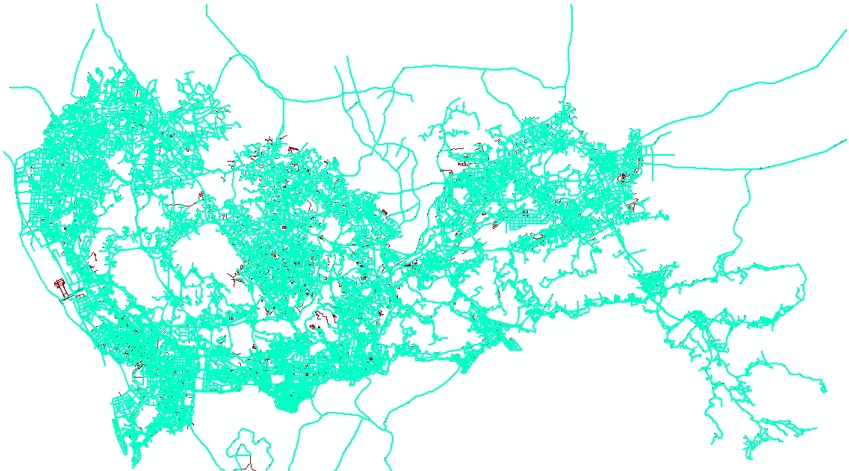
\includegraphics[width=\textwidth]{chp02_2017年度更新道路GIS数据空间分布图.jpg}
  \caption[2017年度更新道路GIS数据空间分布图]{2017年度更新道路GIS数据空间分布图(红色为年度更新路段)\label{fig:2017年度更新道路GIS数据空间分布图}}
\end{figure}

更新前的深圳市交通仿真系统(二期)公交站点 GIS 数据共有个 11615 站点,
本年度更新后共有 12664 个。图\ref{fig:2017年度更新公交站点GIS数据空间分布图}为年度更新公交站点 GIS 数据的空间分布情况。

\begin{figure}[ht]
  \centering
  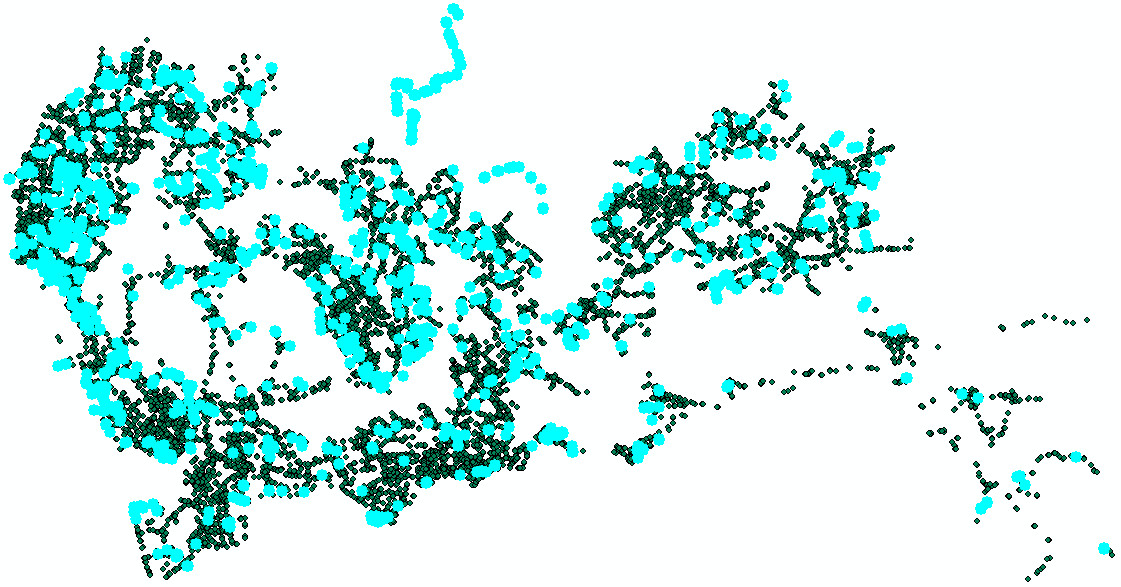
\includegraphics[width=\textwidth]{chp02_2017年度更新公交站点GIS数据空间分布图.jpg}
  \caption[2017年度更新公交站点GIS数据空间分布图]{2017年度更新公交站点GIS数据空间分布图(蓝色为年度更新站点)\label{fig:2017年度更新公交站点GIS数据空间分布图}}
\end{figure}

更新前的深圳市交通仿真系统(二期)公交线路 GIS 数据共有 1877 条(包括上下行),本年度更新后共有 2658 条(包括上下行)。图\ref{fig:2017年度更新公交线路GIS数据空间分布图}为年度更新公交线路 GIS 数据的空间分布情况。

\begin{figure}[ht]
  \centering
  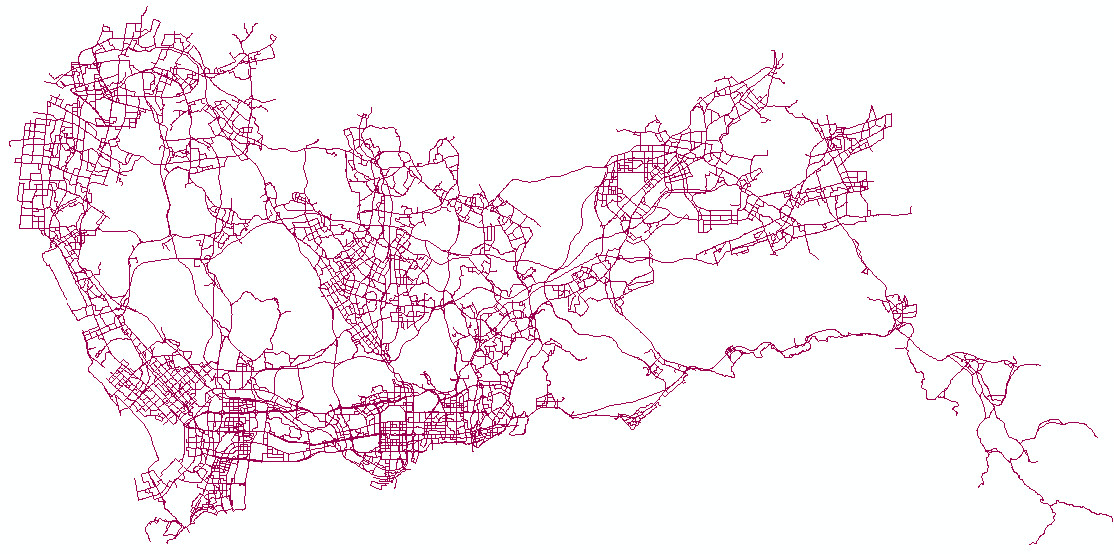
\includegraphics[width=\textwidth]{chp02_2017年度更新公交线路GIS数据空间分布图.jpg}
  \caption{2017年度更新公交线路GIS数据空间分布图\label{fig:2017年度更新公交线路GIS数据空间分布图}}
\end{figure}

% \begin{longtabu} to \textwidth {|X[1,c]|X[1,c]|X[1,c]|X[1.2,c]|X[1.2,c]|}
% \caption{现有静态 GIS 数据\label{tbl:现有静态 GIS 数据}} 
%   \hline
%   \multicolumn{1}{|c|}{\bfseries 类别} & \multicolumn{1}{c|}{\bfseries 名称} &
%   \multicolumn{1}{c|}{\bfseries 格式} & \multicolumn{1}{c|}{\bfseries 主要属性} &
%   \multicolumn{1}{c|}{\bfseries 更新周期} \\\hline
%    & 行政区 & shapefile & 名称、 关内关外 & 由信息中心提供\\\hline
%   \multirow{6}*{基础GIS数据} & 水系 & shapefile & 名称 & 由信息中心提供\\\cline{2-5}
%    & 绿地 & shapefile & 名称 & 由信息中心提供\\\cline{2-5}
%    & 法定图则 & shapefile & 名称 & 由信息中心提供\\\cline{2-5}
%    & 组团 & shapefile & 名称 & 由信息中心提供\\\cline{2-5}
%    & 街道 & shapefile & 名称 & 由信息中心提供\\\cline{2-5}
%    & 人口普查小区 & shapefile & 名称 & 由信息中心提供\\\hline
%    \multirow{5}*{基础路网数据} & 现状道路节点 & shapefile & 坐标、节点类型、所在行政区、所在交通小区、所在街
% 道、所在组团、所在法定图则、交叉口控制类型、立交类型 & 由信息中心提供\\\cline{2-5}
%    & 主要交叉口 & shapefile & 同上 & 不定期  \\\cline{2-5}
%    & 现状道路网络 & shapefile & 起止节点编号、起止道路名称、道路
% 名称、车道数、长度、宽度、机动车道宽度、非机动车道宽度、人行道宽度、 机非分隔带宽
% 度、 中央分隔带宽度、 红线宽度、 道路等级、行车方向、建设方式、 分割类型、 是否具备公交
% 专用道、 交通系统集、 设计车速、 路段通行能力、 路段延误函数、 所在行政区、 所在交通小
% 区、 所在街道、 所在组团、 所在法定图则、 最后更新时间 & 年度 \\\cline{2-5}
%    & 规划道路网络 & shapefile & 同上 & 不定期 \\\cline{2-5}
%    & 交通小区 & shapefile & 形心坐标、所在行政区、所在街道、所在组团、所在法定图则 & 不定期\\\cline{2-5}
% \hline
% \end{longtabu}

